\newpage
%*****************************************************************************
\section{Application to TRACE model of FEBA}\label{sec:gp_application_to_feba}
%*****************************************************************************

In this section, a \gls[hyper=false]{gp} metamodel of the \gls[hyper=false]{trace} model of \gls[hyper=false]{feba} facility is constructed and assessed.
As before, only the results from analyzing \gls[hyper=false]{trace} model of \gls[hyper=false]{feba} test No. $216$ are presented.
Following the results of \gls[hyper=false]{sa} from Chapter 3, only the 12 most influential parameters are being considered in the following.
The resulting \gls[hyper=false]{gp} metamodel of the \gls[hyper=false]{trace} model will then be used for the parameter calibration problem tackled in the next chapter.

%*********************************************************************
\subsection{Simulation Experiment}\label{sub:bc_simulation_experiment}
%*********************************************************************

% Introductory paragraph
The application of the Bayesian calibration framework on the \gls[hyper=false]{trace} reflood model parameters against the \gls[hyper=false]{feba} experimental data is based on $6$ different statistical formulations, in the following referred to as \emph{calibration schemes}.
These schemes are distinguished by their respective assumptions:
\begin{itemize}
	\item \texttt{w/ Bias, All}. The first calibration scheme assumes that the \gls[hyper=false]{trace} model is an imperfect simulator of the reflood phenomena in the \gls[hyper=false]{feba} experiment.
		As such it considers a model \emph{bias} term (as described further below) in the calibration process.
    Furthermore, in this scheme, \emph{all} available types of experimental data are considered.
		The data includes the clad temperature measurements at different time points and at different axial locations (will be succinctly referred to below as the $TC$ output or data),
		the pressure drop measurements at different time points and at different axial segments (referred to as the $DP$ output or data),
		and the collected liquid carryover measurement at different time points (referred to as the $CO$ output or data).
		As mentioned, following the results of the previous chapter, only the most influential $8$ reflood model parameters are considered for the calibration. 
	\item \texttt{w/ Bias, TC}; \texttt{w/ Bias, DP}; and \texttt{w/ Bias, CO} are three variants of the scheme \texttt{w/ Bias, All} in which only one type of experimental data (respectively, output) is considered at a time for the calibration.
		The purpose of these schemes is to investigate the effect of using different types of data from the same test to constrain the model parameters prior uncertainties.
		The calibration is still conducted for the $8$ reflood model parameters and considering the model bias term.
	\item \texttt{w/o Bias} scheme is similar to the scheme \texttt{w/ Bias, All};
		it uses all available types of experimental data to calibrate the $8$ reflood model parameters, except that no model bias term is included in the formulation.
		In essence, this scheme assumes that the \gls[hyper=false]{trace} model perfectly describes the reflood phenomena in the \gls[hyper=false]{feba} test No. $216$.
	\item \texttt{w/ Bias, no dffbVIHT} is the last calibration scheme considered; it is conducted to investigate the effect of excluding, from the calibration process, an influential parameter (\texttt{dffbVIHT}) that is later found from the scheme \texttt{w/ Bias, All} to be strongly correlated.
		Except for calibrating only the $7$ reflood model parameters, this scheme used similar assumptions as the first scheme.
\end{itemize}

The six calibration schemes above aim to update the prior uncertainties of the model parameters using the available experimental data from \gls[hyper=false]{feba} test No. 216.
The six posterior \glspl[hyper=false]{pdf} are then directly sampled using an ensemble \gls[hyper=false]{mcmc} sampler to obtain six different sets of posterior samples.
To avoid the excessive computational cost of having to run \gls[hyper=false]{trace} hundreds of thousands of times, the \gls[hyper=false]{gp} metamodel developed in Chapter~\ref{ch:gp_metamodel} is used to substitute the \gls[hyper=false]{trace} model.

These different sets of samples are then analyzed to assess the effect of using different calibration schemes in constraining the prior uncertainties of the model parameters. 
Finally, the same posterior samples are used in forward \gls[hyper=false]{uq} on the \gls[hyper=false]{trace} model of different \gls[hyper=false]{feba} tests (corresponding to different boundary conditions, namely system pressure and reflood rate).
This final exercise is aimed to assess the implication of the posterior uncertainties from different calibration schemes on (and their applicability for) the prediction under conditions different from the conditions of the calibration data.

In the following, the important terms of Eq.~(\ref{eq:bc_observation_simulation_true}) will be discussed in the context of the present application to the \gls[hyper=false]{trace} model before detailing each calibration scheme.
Afterward, the \gls[hyper=false]{mcmc} sampler as well as a method to evaluate and compare different posterior prediction uncertainties are presented.

%-------------------------------------------------------------------------------------------
\subsubsection{Experimental Data and Observation Layout}\label{subsub:bc_observation_layout}
%-------------------------------------------------------------------------------------------

% Introductory Paragraph
The experimental data of \gls[hyper=false]{feba} test No. $216$ used for the calibration was extracted from the experimental report \cite{Ihle1984} report which was provided to the participants of the \gls[hyper=false]{premium} benchmark \cite{Skorek2013}.

% Clad Temperature
The experimental data provided for the clad temperature ($TC$) of \gls[hyper=false]{feba} test No. $216$ consists of $33$ time points for each of the $8$ different axial locations of the thermocouples along the test section.
\marginpar{Clad temperature ($TC$) data}
Recall that by convention in the experiment, $TC1$ corresponds to the thermocouple measurement at the top of the test section ($\approx 4.1\,[m]$), while $TC8$ corresponds to the measurement at the bottom of the section ($\approx 0.3\,[m]$).

Due to the strong discontinuity of the clad temperature around the point of quenching, the model bias term cannot be modeled using stationary \gls[hyper=false]{gp} (see Section~\ref{subsub:bc_model_bias}) as it severely violates the constant variance assumption as function of time and axial location (at the very least, before and after the quenching occurs).
To keep using a simple stationary \gls[hyper=false]{gp} formulation, the model bias term is modeled only for the part of the transient before the quenching occurs.
Thus, the calibration is also conducted using only the data prior to quenching.
This is further justified by the fact that after quenching there is almost no relevant variation in the temperature transient.

Because of the different timing of quenching along the test section, the number of data points available for calibration changes per axial location.
Based on these data points, an observation layout for $TC$ data can be defined,
\begin{equation}
	\begin{split}
		\boldsymbol{\Lambda}_{TC} & = \{(z_1,t_1),(z_1,t_{2}),(z_2,t_1),\ldots,(z_2,t_{7}),\\
															& \quad\quad (z_3,t_1),\ldots,(z_3,t_{12}),(z_4,t_1),\ldots,(z_4,t_{17}),  \\
															& \quad\quad (z_5,t_1),\ldots,(z_5,t_{21}),(z_6,t_1),\ldots,(z_6,t_{24}),  \\
															& \quad\quad (z_7,t_1),\ldots,(z_7,t_{25}),(z_8,t_1),\ldots,(z_8,t_{27})\} \\
	\end{split}
\label{eq:bc_observation_layout_feba_tc}
\end{equation}
where $z$ denotes the axial location and $t$ denotes the time point.
The total number of data points associated with $TC$ output is $133$.

% Clad Temperature uncertainty
The reported experimental uncertainty associated with the clad temperature measurement is $\pm0.5\%$ of the measured value in $[^oC]$.
In this thesis, this statement of uncertainty is translated to a Gaussian probability distribution such that the uncertainty covers the $99.7\%$ probability (i.e., $3$-$\sigma$ level).
Let $\mathbf{y}_{E,TC}$ be the vector of $TC$ data observed at $\boldsymbol{\Lambda}_{TC}$, then the experimental uncertainty is given as,
\begin{equation}
	\begin{split}
		& \mathcal{E}(\boldsymbol{\Lambda}_{TC}) \thicksim \mathcal{N}(0, \Sigma_{TC})\\
		& \Sigma_{E,TC} = \text{diag}\left(\left(\frac{0.005}{3}\mathbf{y}_{E,TC}\right)^2\right)
	\end{split}	
\label{eq:bc_experimental_uncertainty_feba_tc}
\end{equation}
The dimension of the multivariate Gaussian random variable above is $133$ the length of the observation layout $\boldsymbol{\Lambda}_{TC}$.
The random variable is independent but not identically distributed as the variance changes for each measurement point.

% Pressure Drop
The experimental data provided for the pressure drop ($DP$) of \gls[hyper=false]{feba} test No. $216$ consists of $18$ time points for each of the $4$ different axial segments of the pressure drop measurements.
\marginpar{Pressure drop ($DP$) data}
Recall that in the experiment, the \emph{bottom} segment corresponds to the segment $0.0 - 1.7\,[m]$, the \emph{middle} to $1.7 - 2.3\,[m]$, the \emph{top} to $z = 2.3 - 4.1\,[m]$, and the \emph{total} to $0.0 - 4.1\,[m]$.
In the following, the bottom, middle, top, and total segments are simply indices of the $DP$ output; $z_1$, $z_2$, $z_3$, $z_4$, respectively.
The observation layout for the $DP$ data is then defined as follow,
\begin{equation}
		\boldsymbol{\Lambda}_{DP} = \{(z_1,t_1),\ldots,(z_1,t_{18}),(z_2,t_1),\ldots,(z_4,t_{18})\}
\label{eq:bc_observation_layout_feba_dp}
\end{equation}
where $z$ denotes axial segment and $t$ denotes the time point.
The total length of the observation layout $\boldsymbol{\Lambda}_{DP}$ is $72$.
 
% Pressure drop uncertainty
The reported experimental uncertainty associated with the pressure drop measurement is $\pm10\%$ of the measured value in $[Pa]$.
As before, this statement of uncertainty is translated to a Gaussian probability distribution covering the $99.7\%$ probability (i.e., $3$-$\sigma$ level).
Let $\mathbf{y}_{E,DP}$ is the vector of $DP$ data observed at $\boldsymbol{\Lambda}_{DP}$, then the experimental uncertainty is given as a multivariate Gaussian,
\begin{equation}
	\begin{split}
		& \mathcal{E}(\boldsymbol{\Lambda}_{DP}) \thicksim \mathcal{N}(0, \Sigma_{DP})\\
		& \Sigma_{E,DP} = \text{diag}\left(\left(\frac{0.1}{3}\mathbf{y}_{E,DP}\right)^2\right)
	\end{split}	
\label{eq:bc_experimental_uncertainty_feba_dp}
\end{equation}
where the random variable is a $72$-dimensional multivariate Gaussian.

% Liquid carryover
Finally, the experimental data provided for the liquid carryover ($CO$) of \gls[hyper=false]{feba} test No. $216$ initially consists of $16$ time points.
\marginpar{Liquid carryover ($CO$) data}
However, because the collecting tank was saturated at $10\,[kg]$ only the transient up to that mass is of interest.
By excluding the data points where the tank has been saturated, only $7$ data points are available for the calibration.
Based on these data points $\mathbf{y}_{E,CO}$, the observation layout for the $CO$ data is defined as,
\begin{equation}
		\boldsymbol{\Lambda}_{CO}  = \{(t_1),\ldots,(t_{7})\}
\label{eq:bc_observation_layout_feba_co}
\end{equation}
where $t$ denotes the time point.

% Liquid carryover uncertainty
A large uncertainty was indicated for the liquid carryover measurement that possibly includes biased measurement as the measured mass in the collecting tank does not always correspond to the liquid carryover of the reflood transient \cite{Sanz2017}.
The suggested level of uncertainty for the benchmark was $\pm0.5\,[kg]$.
To cover the reported uncertainty and the possible bias, the reported level is assumed to be $1$-$\sigma$ level of an independent identically distributed multivariate Gaussian,
\begin{equation}
	\begin{split}
		& \mathcal{E}(\boldsymbol{\Lambda}_{CO}) \thicksim \mathcal{N}(0, \mathbf{I} \sigma^2_{CO})\\
	\end{split}
\label{eq:bc_experimental_uncertainty_feba_co}
\end{equation}
where $\mathbf{I}$ is an identity matrix of size $7$, the length of the observation layout $\boldsymbol{\Lambda}_{CO}$ and
$\sigma_{E,CO}$ is the standard deviation of the distribution, taken to be $0.5\,[kg]$.

% Full observation layout
Finally, the observation layout for each output (data) type can be combined into a single long vector of the full observation layout,
$\boldsymbol{\Lambda} = \{\boldsymbol{\Lambda}_{TC}, \boldsymbol{\Lambda}_{DP}, \boldsymbol{\Lambda}_{CO}\}$.
The total number of data points of \gls[hyper=false]{feba} test No. $216$, and the length of the observation layout $\boldsymbol{\Lambda}$, used in the calibration is thus $212$.

%---------------------------------------------------------------------------------------------
\subsubsection{Gaussian Process Approximation for TRACE Simulations}\label{subsub:bc_gp_trace}
%---------------------------------------------------------------------------------------------

Following the results of Chapter~\ref{ch:gp_metamodel}, three separate multivariate \gls[hyper=false]{gp} metamodels are used to approximate the \gls[hyper=false]{trace} predictions for each type of output ($TC$, $DP$, and $CO$).
The hyper-parameters associated with these metamodels are separately estimated using actual \gls[hyper=false]{trace} runs $\mathbf{Y}$ based on a design of experiment $\mathbf{DM}$ (see the details in Section~\ref{sec:gp_application_to_feba}).
After being estimated, the hyper-parameters of the \gls[hyper=false]{gp} metamodel are kept constant in the application of the metamodel.

Under the \gls[hyper=false]{gp} formulation, the simulator prediction for a given input $\bm{x}_o$ (contain both the controllable inputs $\bm{x}_c$ and the model parameters $\bm{x}_m$) becomes a probabilistic model.
The prediction of $TC$ output at the observation layout $\boldsymbol{\Lambda}_{TC}$ is formulated as follows,
\begin{equation}
	\begin{split}
		& \bm{\mathcal{Y}}_{M,TC} (\bm{x}_o) | \mathbf{Y} \sim \mathcal{N} (\boldsymbol{\mu}_{M,TC} (\bm{x}_o), \Sigma_{M,TC} (\bm{x}_o)) \\
		& \boldsymbol{\mu}_{M,TC}  = \bar{\mathbf{y}}_{TC} + \boldsymbol{\Phi}^*_{Q_{TC},TC} \mathbf{m}_{SK,TC}(\bm{x}_o) \\
		& \Sigma_{M,TC} = \boldsymbol{\Phi}^*_{Q_{TC},TC} \text{diag}(\mathbf{s}^2_{SK,TC}(\bm{x}_o)) \boldsymbol{\Phi}^{*T}_{Q,TC} + \boldsymbol{\Phi}^*_{>Q_{TC},TC} \mathbf{I}\boldsymbol{\Phi}^{*T}_{>Q_{TC},TC}) \\
		& \mathbf{m}_{SK,TC} = [m_{SK,TC,1}(\bm{x}_o), m_{SK,TC,2}(\bm{x}_o), \cdots, m_{SK,TC,Q_{TC}}(\bm{x}_o)] \\
		& \mathbf{s}^2_{SK,TC} = [s^2_{SK,TC,1}(\bm{x}_o), s^2_{SK,TC,2}(\bm{x}_o), \cdots, s^2_{SK,TC,Q_{TC}}(\bm{x}_o)]
	\end{split}
\label{eq:p_variate_metamodel_tc}
\end{equation}
where the notations above follow the convention of Section~\ref{sub:gp_multivariate}.
Following the developments in Section~\ref{sec:gp_application_to_feba}, the number of retained principal components for the $TC$ output $Q_{TC}$ is selected to be $7$.

Recall that the \gls[hyper=false]{svd} was conducted on the full \gls[hyper=false]{trace} simulation output (in the case of the temperature output: at $8$ axial levels and at 10'000 time-steps) for the dimension reduction.
However, in the observation layout of Eq.~(\ref{eq:bc_observation_layout_feba_tc}), not all points in time of the full simulation output have corresponding experimental data.
As such, in this chapter for the calibration, the observation layout $\boldsymbol{\Lambda}_{TC}$ is used to select the elements of the output mean vector $\bar{\mathbf{y}}_{TC}$, the eigenvectors $\boldsymbol{\Phi}^*_{Q_{TC},TC}$, and the unretained eigenvectors $\boldsymbol{\Phi}^*_{>Q_{TC},TC}$ such that they contain only the points in time where data are actually observed.
The resulting dimension of the Gaussian distribution is thus $133$.

The formulation for the $DP$ output at the $\boldsymbol{\Lambda}_{DP}$ (Eq.~(\ref{eq:bc_observation_layout_feba_dp})) follows accordingly,
\begin{equation}
	\begin{split}
		& \bm{\mathcal{Y}}_{M,DP} (\bm{x}_o) | \mathbf{Y} \sim \mathcal{N} (\boldsymbol{\mu}_{M,DP} (\bm{x}_o), \Sigma_{M,DP} (\bm{x}_o)) \\
		& \boldsymbol{\mu}_{M,DP}  = \bar{\mathbf{y}}_{DP} + \boldsymbol{\Phi}^*_{Q_{DP},DP} \mathbf{m}_{SK,DP}(\bm{x}_o) \\
		& \Sigma_{M,DP} = \boldsymbol{\Phi}^*_{Q_{DP},DP} \text{diag}(\mathbf{s}^2_{SK,DP}(\bm{x}_o)) \boldsymbol{\Phi}^{*T}_{Q_{DP},DP} + \boldsymbol{\Phi}^*_{>Q_{DP},DP} \mathbf{I}\boldsymbol{\Phi}^{*T}_{>Q,DP}) \\
		& \mathbf{m}_{SK,DP} = [m_{SK,DP,1}(\bm{x}_o), m_{SK,DP,2}(\bm{x}_o), \cdots, m_{SK,DP,Q_{DP}}(\bm{x}_o)] \\
		& \mathbf{s}^2_{SK,DP} = [s^2_{SK,DP,1}(\bm{x}_o), s^2_{SK,DP,2}(\bm{x}_o), \cdots, s^2_{SK,DP,Q_{DP}}(\bm{x}_o)]
	\end{split}
\label{eq:p_variate_metamodel_dp}
\end{equation}
where $Q_{DP}$, the number of retained principal components with respect to the $DP$ output, is taken to be $10$.
As before, the observation layout $\boldsymbol{\Lambda}_{DP}$ is used to select the elements of the output mean vector $\bar{\mathbf{y}}_{DP}$, the eigenvectors $\boldsymbol{\Phi}^*_{Q_{DP},DP}$, and the unretained eigenvectors $\boldsymbol{\Phi}^*_{>Q_{DP},DP}$ such that they contain only the observed points of the $DP$ outputs in time.

Finally, the $CO$ output at the observation layout $\boldsymbol{\Lambda}_{CO}$ (Eq.~(\ref{eq:bc_observation_layout_feba_co})) for a given input $\bm{x}_o$,
\begin{equation}
	\begin{split}
		& \bm{\mathcal{Y}}_{M,CO} (\bm{x}_o) | \mathbf{Y} \sim \mathcal{N} (\boldsymbol{\mu}_{M,CO} (\bm{x}_o), \Sigma_{M,CO} (\bm{x}_o)) \\
		& \boldsymbol{\mu}_{M,CO}  = \bar{\mathbf{y}}_{CO} + \boldsymbol{\Phi}^*_{Q_{CO},CO} \mathbf{m}_{SK,CO}(\bm{x}_o) \\
		& \Sigma_{M,CO} = \boldsymbol{\Phi}^*_{Q_{CO},CO} \text{diag}(\mathbf{s}^2_{SK,CO}(\bm{x}_o)) \boldsymbol{\Phi}^{*T}_{Q_{CO},CO} + \boldsymbol{\Phi}^*_{>Q_{CO},CO} \mathbf{I}\boldsymbol{\Phi}^{*T}_{>Q_{CO},CO}) \\
		& \mathbf{m}_{SK,CO} = [m_{SK,CO,1}(\bm{x}_o), m_{SK,CO,2}(\bm{x}_o), \cdots, m_{SK,CO,Q_{CO}}(\bm{x}_o)] \\
		& \mathbf{s}^2_{SK,CO} = [s^2_{SK,CO,1}(\bm{x}_o), s^2_{SK,CO,2}(\bm{x}_o), \cdots, s^2_{SK,CO,Q_{CO}}(\bm{x}_o)]
	\end{split}
\label{eq:p_variate_metamodel_co}
\end{equation}
where $Q_{CO} = 5$ is the number of retained principal components with respect to the $CO$ output.
Once more, the observation layout $\boldsymbol{\Lambda}_{CO}$ is used to select the elements of the output mean vector $\bar{\mathbf{y}}_{CO}$, the eigenvectors $\boldsymbol{\Phi}^*_{Q_{CO},CO}$, and the unretained eigenvectors $\boldsymbol{\Phi}^*_{>Q_{CO},CO}$ such that they contain only the points in time coincide with the observed data.

%-----------------------------------------------------------------------
\subsubsection{Modeling the Model Bias Term}\label{subsub:bc_model_bias}
%-----------------------------------------------------------------------

% Introductory Paragraph
Following the discussion of Section~\ref{sub:bc_modular_bias}, the model bias term is represented using a \glsfirst[hyper=false]{gp}.
Model bias term is formulated for each type of data (or output).
The formulation of a \glsfirst[hyper=false]{gp} for the model bias term is adapted from \cite{Bayarri2007,Liu2009} (and applied in the reflood model calibration \cite{Wicaksono2016}):
\begin{enumerate}
	\item Generate $N$ realizations of \gls[hyper=false]{trace} simulation for \gls[hyper=false]{feba} test No. $216$ (randomly) varying only the $4$ parameters related to the boundary conditions (namely, \texttt{breakP}, \texttt{fillT}, \texttt{fillV}, and \texttt{pwr}), while keeping the other $8$ model parameters at their respective nominal values.
    Each output type of the \gls[hyper=false]{trace} simulations are selected at its respective observation layout ($\boldsymbol{\Lambda}_{TC}$, $\boldsymbol{\Lambda}_{DP}$, and $\boldsymbol{\Lambda}_{CO}$).
    For each simulation the vectors of values are denoted $\mathbf{\hat{y}}_{M,TC}$, $\mathbf{\hat{y}}_{M,DP}$, and $\mathbf{\hat{y}}_{M,CO}$ for the $TC$, $DP$, $CO$ output, respectively.
  \item Assume the vectors $\left(\mathbf{y}_{E,TC} - \mathbf{\hat{y}}_{M,TC}\right)$, $\left(\mathbf{y}_{E,DP} - \mathbf{\hat{y}}_{M,DP}\right)$, and\\ $\left(\mathbf{y}_{E,CO} - \mathbf{\hat{y}}_{M,CO}\right)$ are realizations from stationary \glspl[hyper=false]{gp} on the observation layouts (i.e., as function time and space). Note as the observation layouts comprise discrete points in time and space, the \glspl[hyper=false]{gp} collapse to multivariate Gaussian distributions.
    The power-exponential covariance function is selected for the covariance kernel and the hyper-parameters of the process (i.e., $\sigma^2$. $\bm{p}$, $\bm{\theta}$) are estimated using the \texttt{R} package \texttt{DiceKriging}. 
  \item The mean of the bias term is taken to be the difference between the data and the nominal prediction, while the covariance matrix of the bias term is taken to be covariance matrix constructed at the observation layout using the estimated hyper-parameters above.
  The constructed covariance matrix takes into account correlations of the model bias in time and space.
  In the present analysis the estimated values of the hyper-parameters above in the previous step are kept constant.
\end{enumerate}

% What does the bias mean
The above model bias term formulation is only partially Bayesian as it uses the data to make the initial estimation.
But as argued in \cite{Bayarri2007} it is a pragmatic way to carry out the analysis as there is no independent data to formulate the bias.
Several additional assumptions are made in this thesis to fully formulate the term.
By varying the parameters related to the boundary conditions in the construction of the term implies that the residual uncertainty of the experiment is included in the model bias term.
The residual uncertainty was not directly observed as no replication at the same controllable inputs was conducted in the experiment. 
In the present analysis, \gls[hyper=false]{trace} simulation is used as a substitute instead. 

By using the above mean for the bias term, any difference between the nominal \gls[hyper=false]{trace} prediction and the experimental data is corrected.
This is an indirect way of putting a strong prior preference for the \gls[hyper=false]{trace} nominal prediction such that the model parameters should not dramatically be shifted to correct the mismatch between the experimental data and the \gls[hyper=false]{trace} prediction.
In other words, it is a way to keep as much as possible the nominal \gls[hyper=false]{trace} prediction which was already based on a long running V\&V activities, but does not include the data from \gls[hyper=false]{feba} experiment in it.
Ref. \cite{Bayarri2007} also recommends that the variance of the process is allowed to vary but as the calibration conducted here is based only on the data from a single \gls[hyper=false]{feba} test, it is decided that the variance is kept constant.
In fact, this represents a pessimistic assumption in the sense that the data is not allowed to reduce the bias by altering the model parameters in line with assuming the mean before.

All in all, the calibration using this proposed model bias term thus aims to update the prior uncertainties of the model parameters assuming that the nominal prediction is centered around the data while keeping the variance unchanged. 
The interest is then emphasized on using experimental data to obtain the uncertainties of the model parameters consistent with these assumptions.

% TC Output
Based on the above discussion, the model bias term for the $TC$ output is expressed as,
\begin{equation}
	\begin{split}
		& \bm{\mathcal{D}}_{TC} \sim \mathcal{N} (\mathbf{m}_{\delta,TC}, \Sigma_{\delta,TC}) \\
		& \mathbf{m}_{\delta,TC} = \left(\mathbf{y}_{E,TC} - \mathbf{\hat{y}}_{M,TC}\right) \\
		& \Sigma_{\delta,TC} = \sigma_{TC}^2 R_{TC}(\boldsymbol{\Lambda}_{TC}, \boldsymbol{\Lambda}_{TC})\ \\
	\end{split}
\label{eq:feba_gp_bias_tc}
\end{equation}
where $\mathbf{m}_{\delta,TC}$ and $\Sigma_{\delta,TC}$ are the mean vector and the covariance matrix of the model bias term with respect to the $TC$ output, respectively;
while $\sigma_{TC}^2$ and $R_{TC}$ are the process variance and correlation function of the process representing the bias term, respectively.
The bias term is a multivariate Gaussian random variable with the dimension dimension of $133$, following the length of the observation layout $\boldsymbol{\Lambda}_{TC}$.

% DP Output
Similarly for the $DP$ output,
\begin{equation}
	\begin{split}
		& \bm{\mathcal{D}}_{DP} \sim \mathcal{N} (\mathbf{m}_{\delta,DP}, \Sigma_{\delta,DP}) \\
		& \mathbf{m}_{\delta,DP} = \left(\mathbf{y}_{E,DP} - \mathbf{\hat{y}}_{M,DP}\right) \\
		& \Sigma_{\delta,DP} = \sigma_{M,DP}^2(\boldsymbol{\Lambda}_{TC}, \boldsymbol{\Lambda}_{TC}) \\
	\end{split}
\label{eq:feba_gp_bias_dp}
\end{equation}
where $\mathbf{m}_{\delta,DP}$ and $\Sigma_{\delta,DP}$ are the mean vector and the covariance matrix of the model bias term with respect to the $DP$ output, respectively;
the terms $\sigma_{DP}^2$ and $R_{DP}$ are the process variance and correlation function of the process representing the bias term, respectively.
According to the length of the observation layout $\boldsymbol{\Lambda}_{DP}$, the multivariate Gaussian random variable above has the dimension of $72$. 

% CO Output
And lastly for the $CO$ output,
\begin{equation}
	\begin{split}
		& \bm{\mathcal{D}}_{CO} \sim \mathcal{N} (\mathbf{m}_{\delta,CO}, \Sigma_{\delta,CO}) \\
		& \mathbf{m}_{\delta,CO} = \left(\mathbf{y}_{E,TC} - \mathbf{\hat{y}}_{M,TC}\right) \\
		& \Sigma_{\delta,CO}  = \sigma_{M,CO}^2(\boldsymbol{\Lambda}_{CO}, \boldsymbol{\Lambda}_{CO})  \\
	\end{split}
\label{eq:feba_gp_bias_co}
\end{equation}
where $\mathbf{m}_{\delta,CO}$ and $\Sigma_{\delta,CO}$ are the mean vector and the covariance matrix of the model bias term with respect to the $CO$ output, respectively;
while $\sigma_{CO}^2$ and $R_{CO}$ are the process variance and correlation function of the process representing the bias term.
The dimension of the multivariate Gaussian random variable above is $7$ following the length of the observation layout $\boldsymbol{\Lambda}_{CO}$.

% Final note
As final note, the formulation of the model bias term is supposed to include explicitly different controllable inputs $\bm{x}_c$ to take into account possible change in the bias as function of the inputs.
However, the present study considers for the calibration only the data from \gls[hyper=false]{feba} test No. $216$ corresponding to a single combination of controllable inputs.
Therefore, the parametrization of $\bm{x}_c$ is dropped from the following notation.

%-----------------------------------------------------------------------
\subsubsection{Calibration Schemes}\label{subsub:bc_calibration schemes}
%-----------------------------------------------------------------------

% Introductory Paragraph
Having defined the elements of the generic calibration formula of Eq.~(\ref{eq:bc_observation_simulation_true}) within the context of the present problem,
the explicit formulation for each calibration scheme introduced in the beginning of this Section can now be presented.

% w/ Bias, TC
The calibration scheme \texttt{w/ Bias, All} combines the formulation of the calibration schemes \texttt{w/Bias, TC}, \texttt{w/Bias, DP}, and \texttt{w/Bias, CO}.
\marginpar{\texttt{w/ Bias, TC}}
As such, in the following the latter three calibration schemes are first presented.
Combining the terms of the above according to Eq.~(\ref{eq:bc_observation_simulation_true}) gives similar formulation as Eq.~(\ref{eq:bc_data_model_gaussian}), but specifically for the $TC$ data generating process.
That is, the process corresponds to the scheme \texttt{w/ Bias, TC},
\begin{equation}
	\begin{split}
		& \bm{\mathcal{Y}}_{E,TC} | \bm{x}_m \sim \mathcal{N} (\boldsymbol{\mu}_{TC} (\bm{x}_m), \Sigma_{TC} (\bm{x}_m)) \\
		& \boldsymbol{\mu}_{TC} (\bm{x}_m) = \boldsymbol{\mu}_{M,TC} (\bm{x}_m) + \mathbf{m}_{\delta,TC} \\
		& \Sigma_{TC} (\bm{x}_m) = \Sigma_{M,TC} (\bm{x}_m) + \Sigma_{\delta,TC} + \Sigma_{E,TC} \\
	\end{split}
\label{eq:likelihood_tc}
\end{equation}
where $\boldsymbol{\mu}_{TC}$ and $\Sigma_{TC} (\bm{x}_m)$ are the $133$-dimensional mean vector and the $133\times 133$ covariance matrix associated with the $TC$ output/data, respectively.
The mean vector $\boldsymbol{\mu}_{TC}$ consists of the mean vector of the \gls[hyper=false]{gp} metamodel prediction $\boldsymbol{\mu}_{M,TC}$ (Eq.~(\ref{eq:p_variate_metamodel_tc}));
and the mean vector of the model bias term $\mathbf{m}_{\delta,TC}$ (Eq.~(\ref{eq:feba_gp_bias_tc})).
The covariance matrix $\Sigma_{TC} (\bm{x}_m)$ comprises the covariance matrix of the \gls[hyper=false]{gp} metamodel prediction (Eq.~(\ref{eq:p_variate_metamodel_tc}));
the covariance matrix of the model bias term $\Sigma_{\delta,TC}$ (Eq.~(\ref{eq:p_variate_metamodel_tc}));
and the covariance matrix of the experimental uncertainty for $TC$ data (Eq.~(\ref{eq:bc_experimental_uncertainty_feba_tc})).

% w/ Bias. DP
In a similar manner, the $DP$ data generating process corresponds to the calibration scheme \texttt{w/ Bias, DP} is as follow
\marginpar{\texttt{w/ Bias, DP}}
\begin{equation}
	\begin{split}
		& \bm{\mathcal{Y}}_{E,DP} | \bm{x}_m \sim \mathcal{N} (\boldsymbol{\mu}_{DP} (\bm{x}_m), \Sigma_{DP} (\bm{x}_m)) \\
		& \boldsymbol{\mu}_{DP} (\bm{x}_m) = \boldsymbol{\mu}_{M,DP} (\bm{x}_m) + \mathbf{m}_{\delta,DP} \\
		& \Sigma_{DP} (\bm{x}_m) = \Sigma_{M,DP} (\bm{x}_m) + \Sigma_{\delta,DP} + \Sigma_{E,DP} \\
	\end{split}
\label{eq:likelihood_dp}
\end{equation}
where $\boldsymbol{\mu}_{DP}$ and $\Sigma_{DP} (\bm{x}_m)$ are the $72$-dimensional mean vector and the $72\times 72$ covariance matrix associated with the $DP$ output/data, respectively.
The mean vector $\boldsymbol{\mu}_{DP}$ consists of the mean vector of the \gls[hyper=false]{gp} metamodel prediction $\boldsymbol{\mu}_{M,DP}$ (Eq.~(\ref{eq:p_variate_metamodel_dp}));
and the mean vector of the model bias term $\mathbf{m}_{\delta,DP}$ (Eq.~(\ref{eq:feba_gp_bias_dp})).
The covariance matrix $\Sigma_{DP} (\bm{x}_m)$ comprises the covariance matrix of the \gls[hyper=false]{gp} metamodel prediction (Eq.~(\ref{eq:p_variate_metamodel_dp}));
the covariance matrix of the model bias term $\Sigma_{\delta,DP}$ (Eq.~(\ref{eq:p_variate_metamodel_dp}));
and the covariance matrix of the experimental uncertainty for $DP$ data (Eq.~(\ref{eq:bc_experimental_uncertainty_feba_dp})).

% w/ Bias, CO
Finally, the $CO$ data generating process corresponds to the calibration scheme \texttt{w/ Bias, CO} is,
\marginpar{\texttt{w/ Bias, CO}}
\begin{equation}
	\begin{split}
		& \bm{\mathcal{Y}}_{E,CO} | \bm{x}_m \sim \mathcal{N} (\boldsymbol{\mu}_{CO} (\bm{x}_m), \Sigma_{CO} (\bm{x}_m)) \\
		& \boldsymbol{\mu}_{CO} (\bm{x}_m) = \boldsymbol{\mu}_{M,CO} (\bm{x}_m) + \mathbf{m}_{\delta,CO} \\
		& \Sigma_{CO} (\bm{x}_m) = \Sigma_{M,CO} (\bm{x}_m) + \Sigma_{\delta,CO} + \Sigma_{E,CO} \\
	\end{split}
\label{eq:likelihood_co}
\end{equation}
where $\boldsymbol{\mu}_{CO}$ and $\Sigma_{CO} (\bm{x}_m)$ are the $7$-dimensional mean vector and the $7\times 7$ covariance matrix associated with the $CO$ output/data, respectively.
The mean vector $\boldsymbol{\mu}_{CO}$ consists of the mean vector of the \gls[hyper=false]{gp} metamodel prediction $\boldsymbol{\mu}_{M,CO}$ (Eq.~(\ref{eq:p_variate_metamodel_tc}));
and the mean vector of the model bias term $\mathbf{m}_{\delta,TC}$ (Eq.~(\ref{eq:feba_gp_bias_co})).
The covariance matrix $\Sigma_{CO} (\bm{x}_m)$ comprises the covariance matrix of the \gls[hyper=false]{gp} metamodel prediction (Eq.~(\ref{eq:p_variate_metamodel_co}));
the covariance matrix of the model bias term $\Sigma_{\delta,CO}$ (Eq.~(\ref{eq:p_variate_metamodel_co}));
and the covariance matrix of the experimental uncertainty for $CO$ data (Eq.~(\ref{eq:bc_experimental_uncertainty_feba_co})).

% w/ Bias, All
The data generating processes for $TC$, $DP$, and $CO$ data above are combined to arrive at the process corresponds to the calibration scheme \texttt{w/ Bias, All}.
\marginpar{\texttt{w/ Bias, All}}
The main assumption in combining the data generating processes is independence between types of data following \cite{Reichert2012}.
That is, no a priori relationship between different types of output is assumed.
This assumption greatly simplifies the problem and thus the joint process becomes a concatenation of the Gaussian random vector 
\begin{equation}
	\begin{split}
		& \bm{\mathcal{Y}}_{E,\{TC,DP,CO\}} | \bm{x}_m \sim \mathcal{N} (\boldsymbol{\mu}_{TC,DP,CP} (\bm{x}_m), \Sigma_{TC,DP,CO} (\bm{x}_m)) \\
		& \boldsymbol{\mu}_{\{TC,DP,CO\}} (\bm{x}_m) = \left[ \boldsymbol{\mu}_{TC} (\bm{x}_m), \boldsymbol{\mu}_{DP} (\bm{x}_m), \boldsymbol{\mu}_{CO} (\bm{x}_m) \right ] \\
		& \Sigma_{\{TC,DP,CO\}} (\bm{x}_m) = \text{diag}(\Sigma_{TC} (\bm{x}_m), \Sigma_{DP} (\bm{x}_m), \Sigma_{CO} (\bm{x}_m)) \\
	\end{split}
\label{eq:likelihood_all}
\end{equation}
where $\boldsymbol{\mu}_{\{TC,DP,CO\}}$ is a $212$-dimensional vector from the concatenation the mean vectors of $TC$, $DP$, and $CO$;
and $\Sigma_{\{TC,DP,CO\}}$ is the $212 \times 212$ covariance matrix.
The $\text{diag}$ operated on matrices results in a block diagonal matrix.
Specifically,
\begin{equation}
   \Sigma_{\{TC,DP,CO\}} (\bm{x}_m) =  
    \begin{pmatrix}
      \Sigma_{TC} (\bm{x}_m)  & \bm{0}_{133\times72}    & \bm{0}_{133\times7}    \\
      \bm{0}_{72\times133}    & \Sigma_{DP} (\bm{x}_m)  & \bm{0}_{72\times7}     \\
      \bm{0}_{7\times133}     & \bm{0}_{7\times72}      & \Sigma_{CO} (\bm{x}_m) \\
    \end{pmatrix}
\label{eq:diag_cov_matrix}
\end{equation} 
Due to the independence assumption between types of data, zero is assigned for the correlations between types of outputs.
Alternatively, due to the same assumption, the density of the joint process is simply the multiplication of the constituent processes.

% w/o Bias
The calibration scheme \texttt{w/o Bias} has a similar data generating process to that of the scheme \texttt{w/ Bias, All},
\marginpar{\texttt{w/o Bias}}
except that the mean vectors and the covariance matrices of the model bias term for each types of data have been removed from the formulation.
Specifically, the vectors (covariance matrices) $\mathbf{m}_{\delta,TC}$ ($\Sigma_{\delta,TC}$), $\mathbf{m}_{\delta,DP}$ ($\Sigma_{\delta,DP}$), and $\mathbf{m}_{\delta,CO}$ ($\Sigma_{\delta,CO}$) are removed from Eqs.~(\ref{eq:likelihood_tc}), (\ref{eq:likelihood_dp}), and (\ref{eq:likelihood_co}), respectively.

% w/ Bias, no dffbVIHT
Lastly, the calibration scheme \texttt{w/ Bias, no dffbVIHT} has the same data generating process as Eq.~(\ref{eq:likelihood_all}), except that the parameter \texttt{dffbVIHT} is not part of $\bm{x}_m$.
\marginpar{\texttt{w/ Bias, no dffbVIHT}}
In discussion below, this also implies that the parameter is assigned no prior probability.

% Likelihood, Prior, Posterior
Given the experimental data $\mathbf{y}_{E,TC}$, $\mathbf{y}_{E,DP}$, and $\mathbf{y}_{E,CO}$ for the $TC$, $DP$, and $CO$ the likelihood functions with respect to each of the calibration schemes above can be defined following Eq.~(\ref{eq:bc_likelihood}).
\marginpar{Likelihood functions}
The likelihood is from the Gaussian density (the formula for the density is given in Appendix~\ref{app:gaussian_vector}).
Note that the model parameters are embedded inside the likelihood function through the mean and the covariance of the \gls[hyper=false]{gp} metamodel prediction.

% Posterior
The posterior \gls[hyper=false]{pdf} is then formulated by assigning the prior \gls[hyper=false]{pdf} for the $8$ (respectively 7 for the scheme \texttt{w/ Bias, no dffbVIHT}) important reflood model parameters $\bm{x}_m$ from Table~\ref{tab:trace_model_parameter_2}.
\marginpar{Posterior PDFs}
The posterior \gls[hyper=false]{pdf} is defined for each of the calibration schemes using the respective likelihood functions.
For instance, the posterior \gls[hyper=false]{pdf} for the model parameters under the calibration scheme \texttt{w/ Bias, TC} up to a constant is written as,
\begin{equation}
  p_{TC}(\bm{x}_m | \mathbf{y}_{E,TC}) \propto \mathcal{L}_{TC}(\bm{x}_m;\mathbf{y}_{E,TC}) \cdot p(\bm{x}_m)
\label{eq:feba_posterior}
\end{equation}
where the likelihood $\mathcal{L}_{TC}$ is the likelihood function associated with the data generating process in Eq.~(\ref{eq:likelihood_tc}).
The five other likelihood functions and posterior \glspl[hyper=false]{pdf} are defined similarly.
Table~\ref{tab:ch5_calibration_schemes} summarizes the different calibration schemes considered in this study.
\begin{table*}[!htbp]\centering
\ra{0.9}
\begin{adjustwidth*}{}{-3cm}
\caption{Bayesian calibration schemes conducted for the \gls[hyper=false]{trace} reflood model parameters against data from \gls[hyper=false]{feba} test No. $216$.}
\label{tab:ch5_calibration_schemes}
\begin{tabular}{@{}clccccrc@{}}\toprule
\multirow{2}{*}{No.} & \multirow{2}{*}{\shortstack[c]{Calibration Scheme}} 	& \multirow{2}{*}{\shortstack[c]{Model Bias\\Term}}	& \multicolumn{3}{c}{Types of Output} & \phantom{a} & \multirow{2}{*}{\shortstack[c]{Reflood Model\\Parameters \footnotesize{(total number)}}} \\
																															  \cmidrule{4-6}
    &                                 					& 						& $TC$				& $DP$     		& $CO$   				&&	\\ \midrule
1   & \texttt{w/ Bias, All}											& \Checkmark  & \Checkmark  & \Checkmark  & \Checkmark  	&& All \footnotesize{($8$)}          				\\
2   & \texttt{w/ Bias, TC}     									& \Checkmark  & \Checkmark	&							&          			&& All \footnotesize{($8$)}           			\\
3   & \texttt{w/ Bias, DP}     									& \Checkmark 	&         		& \Checkmark	&								&& All \footnotesize{($8$)} 								\\
4   & \texttt{w/ Bias, CO}       								& \Checkmark 	& 						& 						& \Checkmark		&& All \footnotesize{($8$)}           			\\
5   & \texttt{w/o Bias}               					&          		& \Checkmark  & \Checkmark  & \Checkmark		&& All \footnotesize{($8$)}	          			\\
6   & \texttt{w/ Bias, no dffbVIHT}             & \Checkmark  & \Checkmark  & \Checkmark  & \Checkmark		&& Excluding \texttt{dffbVIHT} \footnotesize{(7)}\\
\bottomrule
\end{tabular}
\end{adjustwidth*}
\end{table*}

%---------------------------------------------------------------------------------------
\subsubsection{MCMC Simulation using Ensemble Sampler}\label{subsub:bc_calibration_mcmc}
%---------------------------------------------------------------------------------------

% Introductory paragraph
Each calibration scheme above results in a likelihood function, which when combined with the prior \glspl[hyper=false]{pdf} of the model parameters, yield a posterior \glspl[hyper=false]{pdf}.
The $8$-dimensional (respectively $7$ for the \texttt{w/ Bias, no dffbVIHT} scheme) posterior \glspl[hyper=false]{pdf} contain all the information on the model parameters conditional on the experimental data and the assumed prior uncertainties, under the respective assumed calibration scheme.
To characterize the posterior uncertainties of the model parameters, samples are directly generated from the respective posterior \gls[hyper=false]{pdf} by means of \gls[hyper=false]{mcmc} simulation.

% Parallel requirement
Although the use of \gls[hyper=false]{gp} metamodel alleviates the burden of having to run \gls[hyper=false]{trace} directly, evaluating the likelihood function requires an inversion of the covariance matrix.
The computational cost of matrix inversion is still not negligible, especially considering the expected number of evaluations. 
Furthermore, although the \gls[hyper=false]{aies} \gls[hyper=false]{mcmc} algorithm (Algorithm~\ref{alg:aies}) is straightforward to implement, it is not readily applicable for using multiple CPU \cite{Foreman-Mackey2013}.

% EMCEE and RGW
A parallelization of the \gls[hyper=false]{aies} sampler was originally developed and implemented in the python package \texttt{emcee} \cite{Foreman-Mackey2013}.
The main design philosophy of \texttt{emcee} (and its ported \texttt{R} package \texttt{rgw} \cite{Mantz2016} used in this thesis) is that of a \emph{portable} sampler.
That is, the user simply has to code the posterior formulation (the likelihood and the prior) in the respective generic computing environment (\texttt{R} or python), without the need to put the probabilistic model within a new framework\footnote{Such as the approach adopted in the more established \texttt{WinBugs} \cite{Lunn2000}, \texttt{Jags} \cite{Plummer2003}, and \texttt{Stan} \cite{Carpenter2017a}. These samplers, however, has more extensive capabilities for conducting a Bayesian data analysis and tends to be faster as they port the user-specified probabilistic models to a lower level language (e.g., \texttt{C++}). Furthermore, being older, they have a larger and more diverse user base.}.

% Settings used in the simulation
In the present study, $2'000$ iterations are carried out for an ensemble of $1'000$ walkers.
The initial state of the ensemble is a tight random scatter around the nominal model parameter values.
The total number of iterations depends on the convergence of the \gls[hyper=false]{mcmc} simulation (discarding the initialization bias) and the required level of statistical error as detailed in Section~\ref{sec:bc_mcmc_diagnostic}.
For the present study, they are assessed after-the-fact and the results is indeed found to be sufficient.
Meanwhile, there is no clear cut rule for choosing the number of walkers $L$ \cite{Foreman-Mackey2013}.
Larger number of walkers requires more computational cost per iteration but yields more independent samples per iteration.
At the same time, larger number of walkers might cause more of the initial calculations to be discarded as more calculations are required to settle the ensemble in the typical region of the posterior distribution.
A thousand walkers were selected considering the available computational resources at the time of the analysis.

The \gls[hyper=false]{mcmc} simulation for each calibration schemes results in $2\times10^6$ posterior samples of the model parameters.
These samples are then further post-processed to remove the initialization bias and to reduce the autocorrelation among successive iterations.
 
%-------------------------------------------------------------------------------------
\subsubsection{Evaluating Calibration Results}\label{subsub:bc_calibration_evaluation}
%-------------------------------------------------------------------------------------

% Introductory paragraph
The results of the \gls[hyper=false]{mcmc} simulations are set of samples directly drawn from the respective posteriors.
These multivariate samples are visually represented as \emph{corner plot} depicting the joint posterior samples as a set of $1$-dimensional (univariate) and $2$-dimensional (bivariate) marginals of the posterior distribution (see Section~\ref{sub:bc_calibration_results}).
From the univariate marginal of each model parameter posterior uncertainties, the constraining ability of the data and the calibration scheme can be quickly, if not rigorously, assessed.
From the bivariate marginals, the correlation structure between the model parameters, if any, can be also quickly assessed.

% Forward uncertainty quantification
To investigate the implication of the different posterior samples on the prediction, simulation campaigns for forward \gls[hyper=false]{uq} (uncertainty propagation) are conducted on the \gls[hyper=false]{trace} \gls[hyper=false]{feba} model, using different model parameters posterior uncertainties. 
Furthermore, to assess the applicability of posterior uncertainties for the simulation of different conditions from the condition of the calibration experiment, the campaigns are conducted for $5$ additional \gls[hyper=false]{feba} tests.
In other words, these $5$ additional \gls[hyper=false]{feba} tests becomes the validation data sets.
Finally, to investigate the effect of correlated model parameters on the prediction, the campaigns are conducted both with and without considering the correlation structure in the posterior samples.

% Forward uncertainty quantification
The uncertainty propagation campaigns therefore consists of the campaigns on each \gls[hyper=false]{feba} test using model parameters posterior uncertainties derived from different calibration schemes with and without consideration of the correlation among model parameters.
For each of these campaign, actual \gls[hyper=false]{trace} runs are carried out using $1'000$ posterior samples.
Instead of having to come up with a closed form representation of the multivariate posterior distributions, and to explicitly model any possible correlation structure, these samples are directly drawn from the pool of posterior samples obtained from different calibration schemes.
The results of the propagation are represented in series of plots of prediction with the associated uncertainty bands for the three output types ($TC$, $DP$, and $CO$) similar to the ones presented in the result section of Chapter~\ref{ch:trace_reflood}.
From these plots the different propagation campaign can be compared.

% Calibration
At the same time, the numerous plots are unwieldy to deal with.
To circumvent this issue a more quantitative means of aggregating the results of different predictions uncertainties is required.
Although formal Bayesian approaches are available to assess the quality of the prediction using the model parameters posterior uncertainty\footnote{Formal computer model validation metrics, Bayesian or otherwise, is a research topic in its own right, see for instance the validation metrics proposed in \cite{Rebba2006,Rebba2006a,Jiang2008}. Their application is outside the scope of this thesis.}, this thesis adopts a more pragmatic assessment method based on the possibilistic theory proposed in \cite{Baccou2014}.

The aim of the method is to quickly compare the applicability of the different posterior uncertainties in making prediction.
Loosely speaking, the applicability is measured by the width of the prediction uncertainty as well as its coherence (in the most general sense of the word) with experimental data.
Admittedly, the aim concerns less about the inherent correctness of the posterior uncertainties.
The method was applied to synthesize the results of different participants in the context of benchmarking, namely \gls[hyper=false]{bemuse} \cite{Baccou2014} and \gls[hyper=false]{premium} \cite{Sanz2017} projects. 
The method consists of three steps: \emph{information modeling}, \emph{information evaluation}, and \emph{information synthesis}.
For the comparison purpose in this thesis, only the first two steps above are applied and discussed in the following.

% Information modeling
In the information modeling, the information in a prediction uncertainty of a \gls[hyper=false]{qoi} $y$ is represented by an interval (lower and upper bounds: $LUB_y$ and $UUB_y$, respectively) and a reference value $y_\text{ref.}$.
A \emph{source} of information $src$ for a particular \gls[hyper=false]{qoi} $y$ consists of such an interval and, optionally, a reference value.
If only the interval given by $LUB_y$ and $UUB_y$ is supplied then a rectangular model applies,
\begin{equation}
		\pi_{src,y} (y) = 
			\begin{cases}
				1.0, &  LUB_y \leq y \leq UUB_y \\
			  0.0, & \text{otherwise}
	\end{cases}
\label{eq:calibinfo_rectangular}
\end{equation}
where $\pi$ is the possibility measure, whose minimum and maximum are $0.0$ and $1.0$, respectively.
The rectangular model is used to represent to complete ignorance $\pi_{ign,y}$ in the following.

The presence of a reference value $y_\text{ref.}$ within that intervals allows the triangular model to be defined,
\begin{equation}
  \pi_{src,y} (y) = 
			\begin{cases}
				\frac{y - LUB}{y_\text{ref.} - LUB}, &  LUB \leq y < y_\text{ref.} \\
        \frac{UUB - y}{UUB - y_\text{ref.}}, &  y_\text{ref.} \leq y \leq UUB \\
			  0.0                                , & \text{otherwise}
	\end{cases}
\label{eq:calibinfo_triangular}
\end{equation}
These two information models are illustrated in Fig.~\ref{fig:ch5_calibinfo_modeling}.
\normdoublefigure[pos=tbhp,
                  mainlabel={fig:ch5_calibinfo_modeling},
                  maincaption={Information modeling to represent uncertainty propagation results for a \gls[hyper=false]{qoi} $y$.},%
									mainshortcaption={Information modeling to represent uncertainty propagation results for a QoI $y$.},
                  leftopt={width=0.375\textwidth},
                  leftlabel={fig:ch5_calibinfo_modeling_rectangular},
                  leftcaption={Rectangular model},
                  %leftshortcaption={},%
                  rightopt={width=0.375\textwidth},
                  rightlabel={fig:ch5_calibinfo_modeling_triangular},
                  rightcaption={Triangular model},
                  %rightshortcaption={},
                  %spacing={\hfill}
                 ]
{../figures/chapter5/figures/calibinfo_rectangular}
{../figures/chapter5/figures/calibinfo_triangular}

% Information Evaluation, Informativeness
The information evaluation part of the method comprises two indices to evaluate the quality of information in a given source.
\emph{Informativeness}, associated with a source $src$ and a \gls[hyper=false]{qoi} $y$ is defined as,
\begin{equation}
  \text{Inf}(src, y) = \frac{|\pi_{\text{ign}, y}| - |\pi_{\text{src},y}|}{|\pi_{\text{ign},y}|} = 1 - \frac{1}{2} \frac{UUB - LUB}{UUB_{\text{max.}} - LUB_{\text{min.}}}
\label{eq:informativeness}
\end{equation}
where $|\circ|$ denotes the area under an information model.
Informativeness measures the precision of the uncertain prediction, regardless the position of the reference value within the bound;
it takes value between $0.5$ (the widest uncertainty range of a source, the same as the maximum and minimum bounds) and $1.0$ (the narrowest uncertainty range of a source, practically $0$).
Fig.~\ref{fig:ch5_calibinfo_informativeness} illustrates $\text{Inf}$ calculation.
\normdoublefigure[pos=tbhp,
                  mainlabel={fig:ch5_calibinfo_informativeness},
                  maincaption={Informatives of two different information source. Wider uncertainty interval gives lower informativeness, and vice versa. Thus $\text{Inf}(src_1, y) > \text{Inf}(src_2, y)$},%
									mainshortcaption={Informativeness of two different information sources.},
                  leftopt={width=0.425\textwidth},
                  leftlabel={fig:ch5_calibinfo_informativeness_narrow},
                  leftcaption={Narrower prediction uncertainty},
                  %leftshortcaption={},%
                  rightopt={width=0.425\textwidth},
                  rightlabel={fig:ch5_calibinfo_informativeness_wide},
                  rightcaption={Wider prediction uncertainty},
                  %rightshortcaption={},
                  %spacing={\hfill}
                 ]
{../figures/chapter5/figures/calibinfo_informativeness_narrow}
{../figures/chapter5/figures/calibinfo_informativeness_wide}

% Information Evaluation, Calibration Score
\emph{Calibration score} between a source $src$ and the observed value $y_\text{obs.}$ for a \gls[hyper=false]{qoi} is defined as,
\begin{equation}
  \text{Cal}(src, y) = \pi_{src, y}(y_\text{obs.})
\label{eq:calibration_score}
\end{equation}
that is, the calibration score is the possibility of the observed value $y_\text{obs.}$ under the information model of the source $src$.
It measures the discrepancy between the observed value and uncertain prediction represented by an interval and a reference value.
Following Eq.~(\ref{eq:calibinfo_triangular}), the score severely penalizes the observed data that falls outside the prediction interval; assigning calibration score of $0.0$.
The score is at maximum of $1.0$ for $y_\text{obs.} = y_\text{ref.}$.
It does not, however, takes into account the possible uncertainties associated with $y_\text{obs.}$.
\bigtriplefigure[pos=tbhp,
								 mainlabel={fig:ch5_calibinfo_calib},
			           maincaption={Calibration scores of three different sources with the same observed data $y_\text{obs.}$: $\text{Cal}(src_1, y) > \text{Cal}(src_2, y) > \text{Cal}(src_3, y)$},
			           mainshortcaption={Calibration scores of three different sources with the same observed data $y_\text{obs.}$.},%
			           leftopt={width=0.30\textwidth},
			           leftlabel={fig:ch5_calibinfo_calib1},
			           leftcaption={$\text{Cal}(src_1, y) \approx 1.0$},
			           midopt={width=0.30\textwidth},
			           midlabel={fig:ch5_calibinfo_calib2},
			           midcaption={$\text{Cal}(src_2, y)$},
			           rightopt={width=0.30\textwidth},
			           rightlabel={fig:ch5_calibinfo_calib3},
			           rightcaption={$\text{Cal}(src_3, y) = 0$},
			           spacing={},
			           spacingtwo={}]
{../figures/chapter5/figures/calibinfo_calib1}
{../figures/chapter5/figures/calibinfo_calib2}
{../figures/chapter5/figures/calibinfo_calib3}

% Aggregation
For multiple outputs $\mathbf{y} = [y_1, \ldots, y_D]$ of the same source, both informativeness and calibration score can be aggregated by,
\begin{equation}
  \text{Inf}(src) = \frac{1}{D} \sum_{d=1}^{D} Inf(src, y_d) \quad\quad \text{Cal}(src) = \frac{1}{D} \sum_{d=1}^{D} \text{Cal}(src, y_d)
\label{eq:calibinfo_aggregate}
\end{equation}

% From Probabilistic to Possibilistic
Translating from the Bayesian (probabilistic) framework, the bounds of the prediction interval of the above $LUB$ and $UUB$ can be taken to be two percentiles of the prediction probability distribution that cover a selected probability.
\marginpar{Application of the method}
For instance, the criteria used in the present study, selecting a symmetric $95\%$ probability interval implies the $LUB$ and $UUB$ to be the $2.5$-th and $97.5$-th percentiles, respectively.
The choice is rather arbitrary but as long as the criteria is applied consistently across different prediction uncertainties, the value of the method for comparison is preserved.
Furthermore, the $2.5$-th and $97.5$-th percentiles of the prior prediction distribution are taken to be the $LUB_{\text{min.}}$ and $UUB_{\text{max.}}$ and the reference value $y_\text{ref.}$ is taken to be the median value of each posterior prediction distribution.
Finally the experimental data is taken to be the observed value $y_\text{obs.}$ without considering the associated uncertainty following the original paper \cite{Baccou2014}.
Once again, this lack of consideration is less of an issue for comparing between different uncertain prediction.
 

%*************************************************************************************
\subsection{Dimension Reduction by \glsfirst[hyper=false]{pca}}\label{sub:gp_feba_pca}
%*************************************************************************************

% Introductory paragraph
As mentioned, the different outputs considered in this study (i.e., clad temperature, pressure drop, and liquid carryover) were of multivariate nature.
For instance, the clad temperature output was defined both in time instance and axial location.
Considering eight different axial locations for the thermocouples and $1'000 \, [s]$ transient (to ensure that all runs were quenched) with time step size of $0.1 \, [s]$, the dimensionality of this output amounted to $80'000$.
Fig.~\ref{fig:ch4_plot_image_tc_run} shows three different clad temperature outputs from three different \gls[hyper=false]{trace} runs.
It shows the contour plot of clad temperature as function of time and axial location in the $x$- and $y$- axes, respectively.
Though not shown here, the other two types of output were of similar nature: pressure drop was also defined in time instance and in four axial segments (with dimensionality of the output amounting to $40'000$), while liquid carryover output was defined only in time (with dimensionality amounting to $10'000$).
\bigtriplefigure[pos=tbhp,
                 mainlabel={fig:ch4_plot_image_tc_run},
			           maincaption={Examples of multivariate clad temperature output $[K]$ at eight different locations as function of time, presented as ``images'', taken from three different training runs.},
			           mainshortcaption={Examples of multivariate clad temperature output in at eight different locations as function of time, presented as ``images''},%
			           leftopt={width=0.305\textwidth},
			           leftlabel={fig:ch4_plot_image_tc_run_1},
			           leftcaption={Training run 996},
			           midopt={width=0.305\textwidth},
			           midlabel={fig:ch4_plot_image_tc_run_2},
			           midcaption={Training run 1480},
			           rightopt={width=0.305\textwidth},
			           rightlabel={fig:ch4_plot_image_tc_run_3},
			           rightcaption={Training run $1805$},
			           spacing={},
			           spacingtwo={}]
{../figures/chapter4/figures/plotImageTCRun1}
{../figures/chapter4/figures/plotImageTCRun2}
{../figures/chapter4/figures/plotImageTCRun3}

% Multivariate Clad Temperature
\gls[hyper=false]{pca} was used to reduce this significant number of output dimensions.
Fig.~\ref{fig:ch4_plot_pca_image} shows the sample mean surface and the first two \glspl[hyper=false]{pc} (loadings) estimated using $1'920$ training samples.
These two \glspl[hyper=false]{pc} explained about $83\%$ of the output variance in training samples.
This implied that any realization of the training samples could be reconstructed by using the mean surface 
added by linear combination of the \gls[hyper=false]{pc} multiplied by a unique set of scalars (the standardized \gls[hyper=false]{pc} scores) associated with that realization, such that on average (over many realizations) the reconstruction would be $83\%$ accurate with respect to the \gls[hyper=false]{rmse}.
In other words, ``images'' in Fig.~\ref{fig:ch4_plot_image_tc_run} can be reconstructed by overlapping the mean surface and the multiples of \glspl[hyper=false]{pc} ``images'' shown in Fig.~\ref{fig:ch4_plot_pca_image}.
\bigtriplefigure[pos=tbhp,
                 mainlabel={fig:ch4_plot_pca_image},
			           maincaption={PCA results for the clad temperature output},
			           mainshortcaption={PCA results for the clad temperature output},%
			           leftopt={width=0.29\textwidth},
			           leftlabel={fig:ch4_plot_pca_image_ave},
			           leftcaption={Mean surface},
			           midopt={width=0.29\textwidth},
			           midlabel={fig:ch4_plot_pca_image_pc1},
			           midcaption={$1$\textsuperscript{st} PC loading ($73\%$)},
			           rightopt={width=0.29\textwidth},
			           rightlabel={fig:ch4_plot_pca_image_pc2},
			           rightcaption={$2$\textsuperscript{nd} PC loading ($10\%$)},
			           spacing={},
			           spacingtwo={}]
{../figures/chapter4/figures/plotPCAImageAve}
{../figures/chapter4/figures/plotPCAImagePC1}
{../figures/chapter4/figures/plotPCAImagePC2}

% RMSE of PCA, different output
Fig.\ref{fig:ch4_plot_reconstruction_error} summarizes the convergence behavior of the reconstruction error for the three types of output with increasing number of \glspl[hyper=false]{pc} (up to the first $10$, out of $80'000$, $40'000$, and $10'000$ \glspl[hyper=false]{pc} obtained for the respective outputs) used for the reconstruction.
The plots were obtained from reconstructing the outputs in the validation data set (with sample size of $5'000$) using a set of \glspl[hyper=false]{pc} derived from the training data set and by computing the average of the squared error over all realizations in the validation data set.
\bigtriplefigure[pos=tbhp,
                 mainlabel={fig:ch4_plot_reconstruction_error},
			           maincaption={The reconstruction error, in terms of \gls[hyper=false]{rmse}, as a function of the number of \glspl[hyper=false]{pc} used in the reconstruction of the output space for three different output types.},
			           mainshortcaption={Convergence of the reconstruction error as function of the number of \gls[hyper=false]{pc} used in the reconstruction of the output space for three different output types.},%
			           leftopt={width=0.28\textwidth},
			           leftlabel={fig:ch4_plot_reconstruction_error_tc},
			           leftcaption={Clad temperature output},
			           midopt={width=0.28\textwidth},
			           midlabel={fig:ch4_plot_reconstruction_error_dp},
			           midcaption={Pressure drop output},
			           rightopt={width=0.28\textwidth},
			           rightlabel={fig:ch4_plot_reconstruction_error_co},
			           rightcaption={Liquid carryover output},
			           spacing={},
			           spacingtwo={}]
{../figures/chapter4/figures/plotReconstructionErrorTC}
{../figures/chapter4/figures/plotReconstructionErrorDP}
{../figures/chapter4/figures/plotReconstructionErrorCO}

Because the \gls[hyper=false]{pc} scores used in the reconstruction were exact, the plot shows the magnitude of error to be expected from the dimension reduction procedure for each type of outputs.
It also shows that the benefit of using larger number of \gls[hyper=false]{pc} is increasingly marginal.

%*****************************************************************************************************************************************************************
\subsection{\gls[hyper=false]{gp} \gls[hyper=false]{pc} Metamodel Construction: Training, Validation, and Selection}\label{sub:gp_feba_pca_metamodel_construction}
%*****************************************************************************************************************************************************************

% Introductory paragraph
Following the \gls[hyper=false]{pca} of the multivariate output, 
\gls[hyper=false]{gp} metamodels were constructed with respect to the standardized \gls[hyper=false]{pc} scores for each of the output types.
The effect of several factors potentially affecting the predictive performance of \gls[hyper=false]{gp} metamodel were also investigated, including training sample size as well as the choice of experimental design and covariance kernel function.

% PC GP Metamodel, Clad Temperature Output
It was found that higher \glspl[hyper=false]{pc} tends to be harder to fit.
\marginpar{\gls[hyper=false]{gp} \gls[hyper=false]{pc} metamodel, clad temperature output}
That is, more and more training samples were required to have a \gls[hyper=false]{gp} metamodel of good predictive accuracy.
Fig.~\ref{fig:ch4_plot_pc_q2_tc} shows the predictivity coefficient $Q_2$ as function of training samples for 3 different \glspl[hyper=false]{pc} \gls[hyper=false]{gp} metamodels with respect to the clad temperature output.
The $Q_2$ was calculated based on the validation dataset of size $5'000$ data points (i.e., independent \gls[hyper=false]{trace} runs.
Multiple points per training sample size correspond to \gls[hyper=false]{gp} metamodels constructed using different experimental designs and covariance kernel functions, as well as the multiple replications for each experimental design.
\bigfigure[pos=!tbhp,
					 opt={width=0.9\textwidth},
           label={fig:ch4_plot_pc_q2_tc},
           shortcaption={Convergence of \gls[hyper=false]{pc} metamodel with increasing number of training samples with respect to the standardized \glspl[hyper=false]{pc} scores associated with the clad temperature output}]
{../figures/chapter4/figures/plotPCQ2TC}
{Convergence of \gls[hyper=false]{pc} metamodel with increasing number of training samples with respect to the standardized \glspl[hyper=false]{pc} scores associated with the clad temperature output and $Q_2$ validation metric. The first $10$ \glspl[hyper=false]{pc} contained about $96\%$ of the total clad temperature output variation.
}

The leftmost panel of the plot shows that indeed the \gls[hyper=false]{gp} metamodel for the first standardized \gls[hyper=false]{pc} score is the easiest to fit,
requiring only small number of training samples.
On the other hand, the rightmost panel of the plot shows that not even the largest number of training samples considered is enough to have a \gls[hyper=false]{gp} metamodel with decent performance.
Furthermore, the plot also shows that the variations in the performance tends to become smaller with increasing sample size.

% (negative and zero predictivity coefficient means that no benefit is gained from using \gls[hyper=false]{gp} metamodel to make the prediction)

% PC GP Metamodel Construction, Clad Temperature Output
\begin{sidewaysfigure}
	\centering
	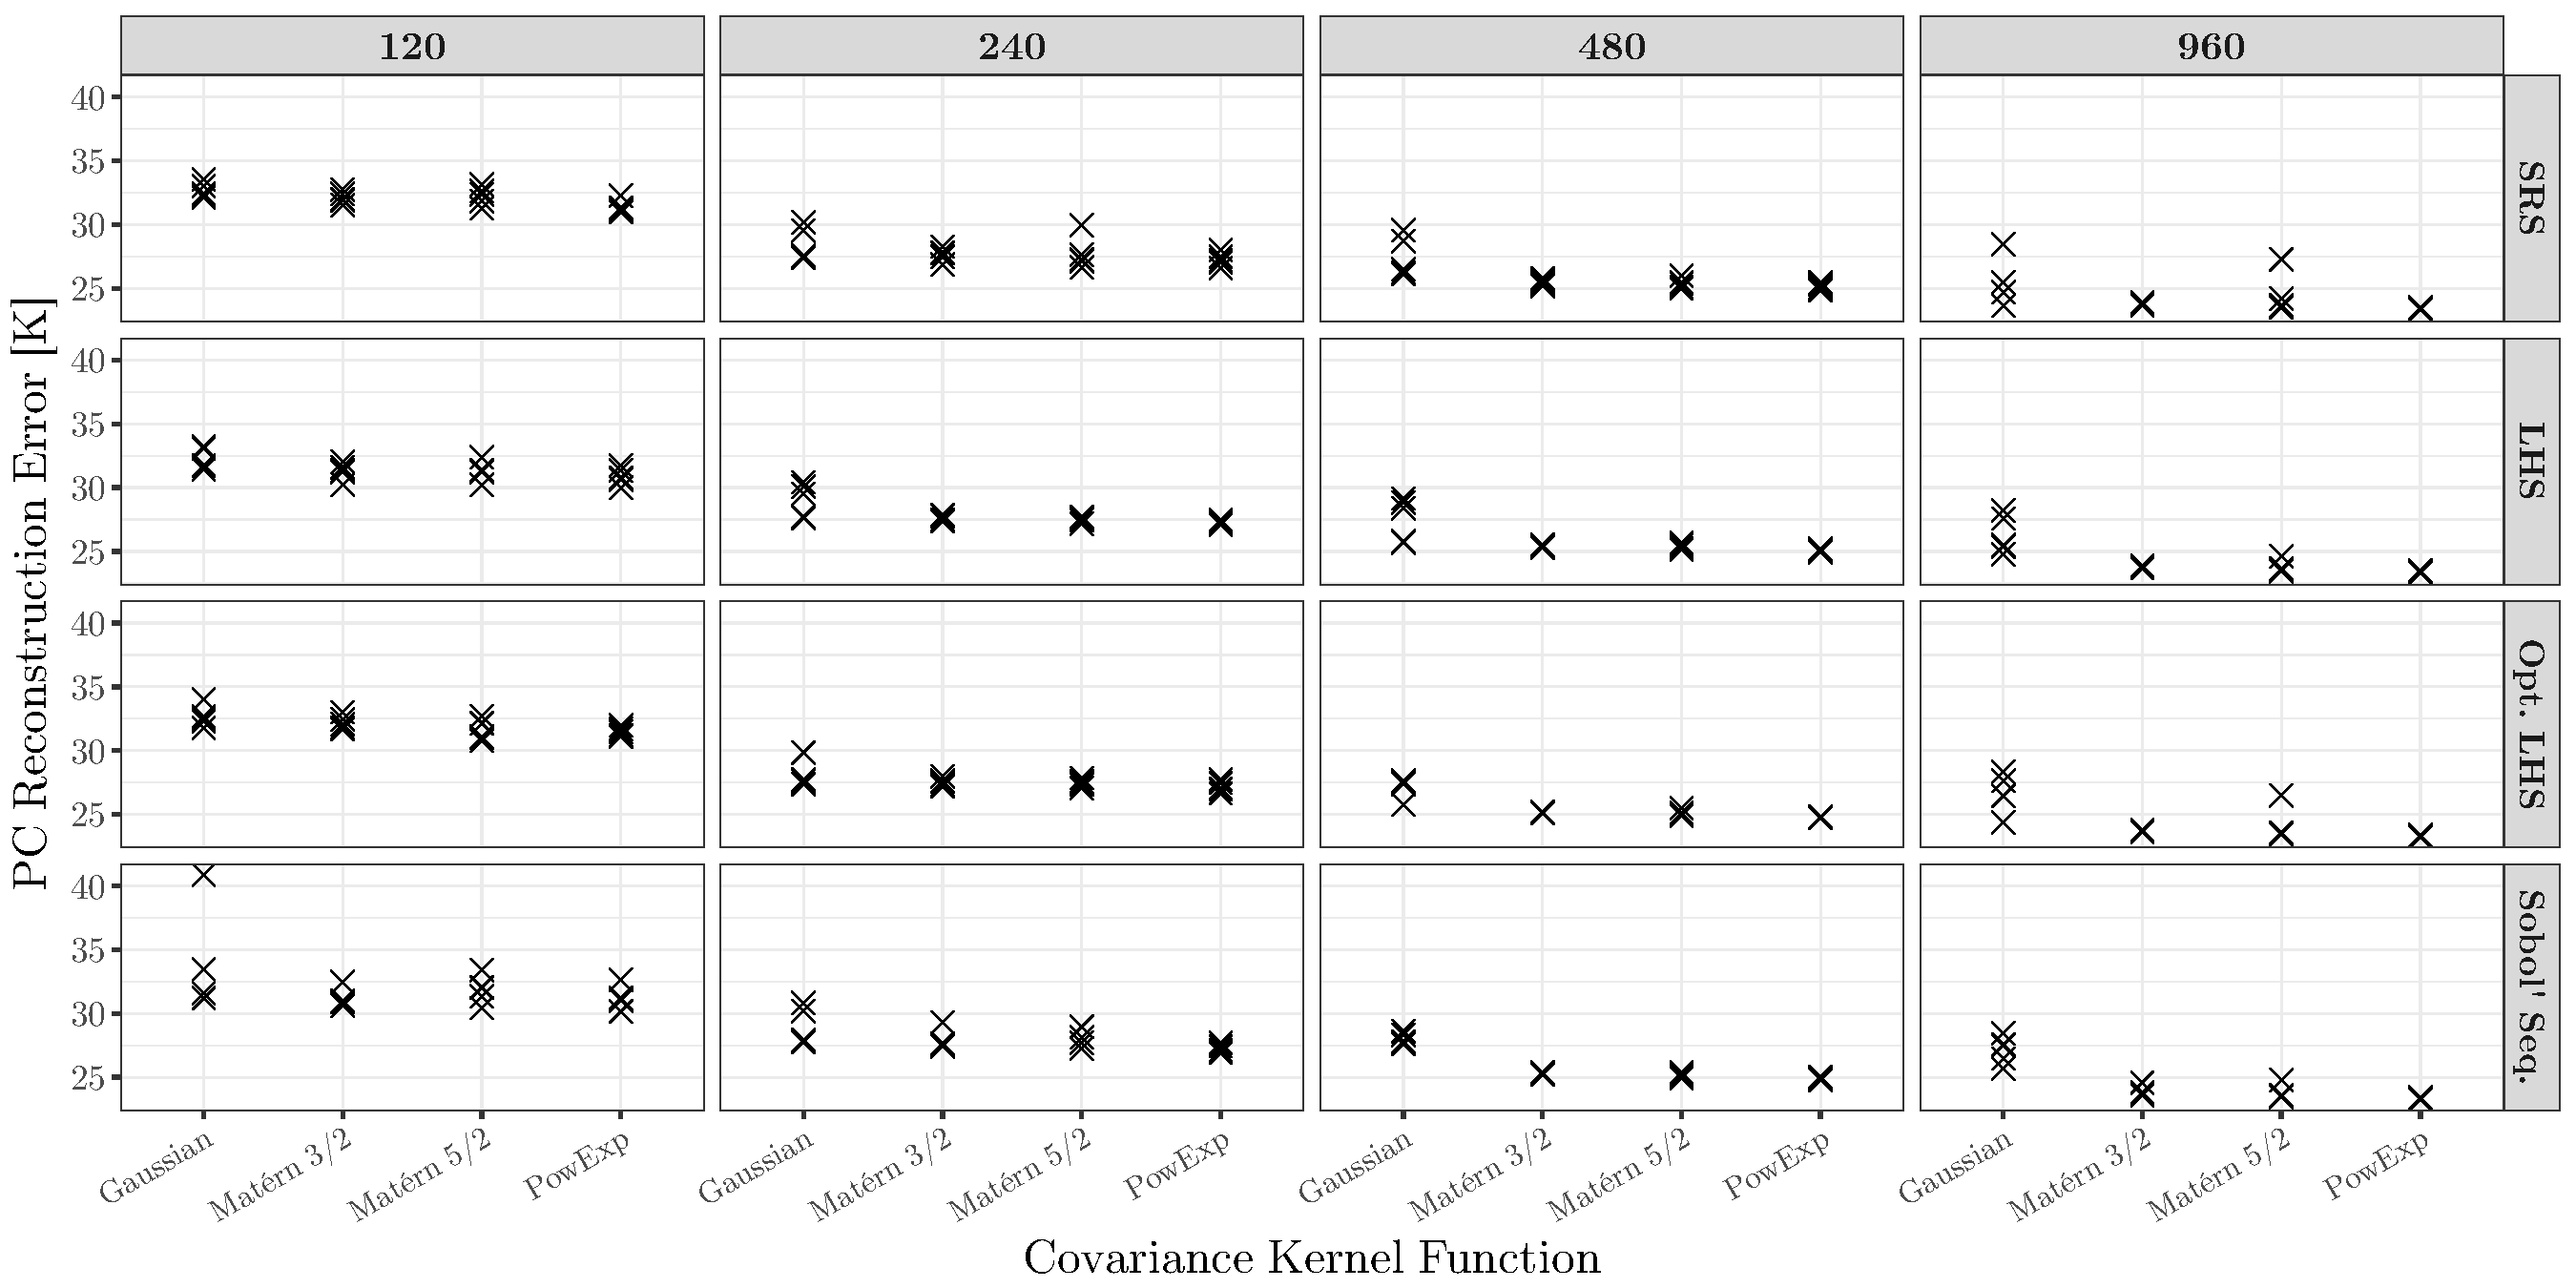
\includegraphics[width=1.0\textwidth]{../figures/chapter4/figures/plotPCGPConstructionTC}
	\caption[The effect of training sample size, experimental design, and covariance function on the predictive performance of GP PC metamodel with respect to the clad temperature output]{The effect of training sample size, experimental design, and covariance function on the predictive performance (in terms of \gls[hyper=false]{rmse}, of \gls[hyper=false]{gp} \gls[hyper=false]{pc} metamodel with respect to the clad temperature output.}
	\label{fig:ch4_plot_pc_gp_construction_tc}
\end{sidewaysfigure}

% Describing the figure itself (as it is the first time it appears)
Fig.~\ref{fig:ch4_plot_pc_gp_construction_tc} summarizes the effect of different training sample sizes, types of experimental design, and types of covariance kernel function on the predictive performance of the constructed \gls[hyper=false]{gp} \gls[hyper=false]{pc} metamodels to predict the clad temperature output.
The training samples were replicated $5$ times for each size and for each design.
The predictive performance was assessed in terms of the \gls[hyper=false]{rmse} which was computed by retaining the first $7$ \glspl[hyper=false]{pc} and it was also based on the same validation dataset.
As such the \gls[hyper=false]{rmse} shown in the figure represents the combined error due to \gls[hyper=false]{pc} truncation and misprediction of the standardized \gls[hyper=false]{pc} scores.

% Describing the finding in the figure
It was found that the size of the training sample was the most important factor in determining the predictive performance of a \gls[hyper=false]{gp} \gls[hyper=false]{pc} metamodel.
The choice of covariance function had some effects on the perfomance especially between the smoother covariance functions (i.e., the Gaussian and the Mate\'rn $5/2$) and the less smooth ones (i.e, the power exponential and the Mate\'rn $3/2$).
\gls[hyper=false]{gp} metamodel constructed using the Gaussian covariance kernel function, in particular,
exhibited significant variation in the performance one training sample replication to another compared to the other covariance kernel functions.
Finally, the choice of experimental design for the training sample was found to have a negligible effect on the predictive performance of the \gls[hyper=false]{gp} metamodel.

% The Pressure Drop Output
The \gls[hyper=false]{gp} \gls[hyper=false]{pc} metamodel to predict the pressure drop output also showed the same behavior of being more and more difficult to fit the higher \glspl[hyper=false]{pc} (See Fig.~\ref{fig:ch4_plot_pc_q2_dp}).
\marginpar{\gls[hyper=false]{gp} \gls[hyper=false]{pc} metamodel, pressure drop output}
The \gls[hyper=false]{gp} metamodel for the first standardized \gls[hyper=false]{pc} score remained the easiest to fit.
However, it was also found that the metamodel of the higher \gls[hyper=false]{pc} had a much better convergence property.
That is,
a metamodel with a decent predictive performance could be obtained to predict the standardized \gls[hyper=false]{pc} score as high as the $10$\textsuperscript{th} \gls[hyper=false]{pc} using the considered sample sizes.
The first $10$ \glspl[hyper=false]{pc}, in turn, carried close to $100\%$ of the total output variation.
\bigfigure[pos=!tbhp,
					 opt={width=0.92\textwidth},
           label={fig:ch4_plot_pc_q2_dp},
           shortcaption={Convergence of \gls[hyper=false]{pc} metamodel with increasing number of training samples with respect to the standardized \glspl[hyper=false]{pc} scores associated with the pressure drop output}]
{../figures/chapter4/figures/plotPCQ2DP}
{Convergence of \gls[hyper=false]{pc} metamodel with increasing number of training samples with respect to the standardized \glspl[hyper=false]{pc} scores associated with the pressure drop output and $Q_2$ validation metric.}

% PC GP Metamodel Construction, Pressure Drop Output
\clearpage
\begin{sidewaysfigure}
	\centering
	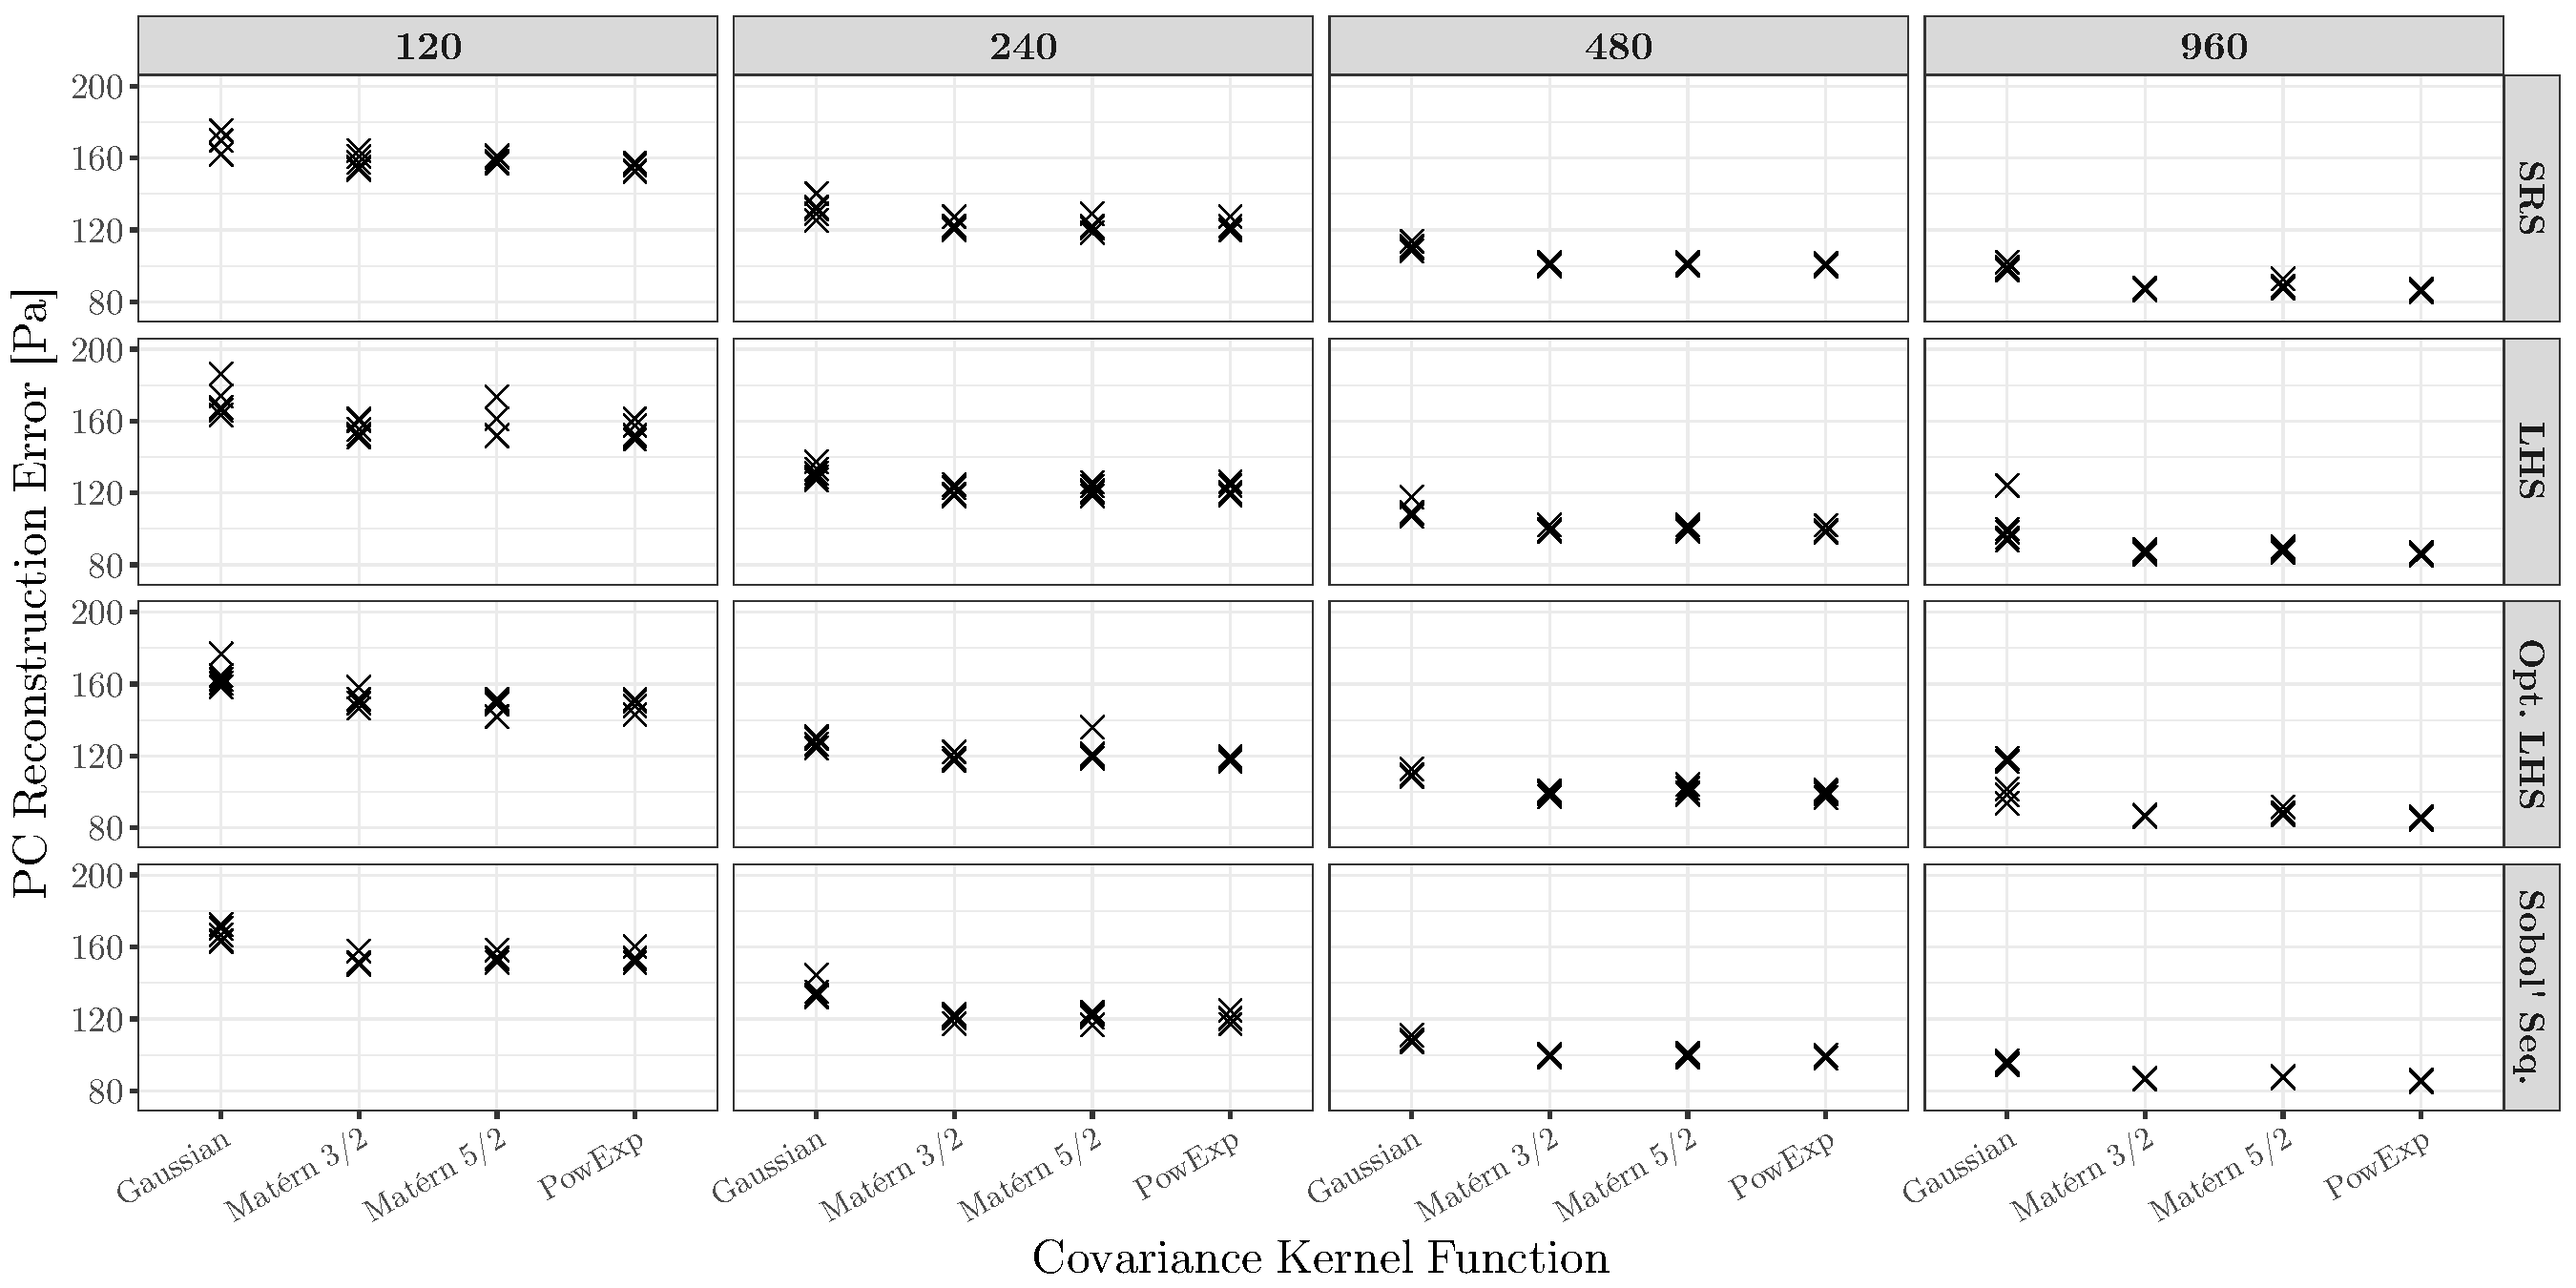
\includegraphics[width=1.0\textwidth]{../figures/chapter4/figures/plotPCGPConstructionDP}
	\caption[The effect of training sample size, experimental design, and covariance function on the predictive performance of GP PC metamodel with respect to the pressure drop output]{The effect of training sample size, experimental design, and covariance function on the predictive performance (in terms of \gls[hyper=false]{rmse}, of \gls[hyper=false]{gp} \gls[hyper=false]{pc} metamodel with respect to the pressure drop output.}
	\label{fig:ch4_plot_pc_gp_construction_dp}
\end{sidewaysfigure}
\clearpage

% Describing finding in the figure, pressure drop output
Fig,~\ref{fig:ch4_plot_pc_gp_construction_dp} presents the summary of the effect of different factors in the construction of a \gls[hyper=false]{gp} metamodel with the pressure drop output as its output.
The reconstruction error was computed using the first $10$ \glspl[hyper=false]{pc}.
The findings were mostly consistent with the previous results for the clad temperature output.
The Gaussian covariance kernel function, as before, had the least stable performance across replication especially when combined with latin hypercube type of experimental design.
Except for that, most of the factors considered converged to the same value of the reconstruction error with less variation across replication compared to the clad temperature output.

% The Liquid carryover output
Finally, the liquid carryover output was found to be even easier to construct compared to the other two types of output.
\marginpar{\gls[hyper=false]{gp} \gls[hyper=false]{pc} metamodel, liquid carryover output}
The first $5$ \glspl[hyper=false]{pc} contained almost all of the total output variation ($\approx 100\%$).
Furthermore, the predictive performance of the \gls[hyper=false]{gp} metamodel converged faster across the first $5$ standardized \gls[hyper=false]{pc} scores (see Fig.~\ref{fig:ch4_plot_pc_q2_co}). 
\bigfigure[pos=!tbhp,
					 opt={width=1.0\textwidth},
           label={fig:ch4_plot_pc_q2_co},
           shortcaption={Convergence of \gls[hyper=false]{gp} metamodel with increasing number of training samples with respect to the standardized \glspl[hyper=false]{pc} scores associated with the liquid carryover output}]
{../figures/chapter4/figures/plotPCQ2CO}
{Convergence of \gls[hyper=false]{gp} metamodel with increasing number of training samples with respect to the standardized \glspl[hyper=false]{pc} scores associated with liquid carryover output and $Q_2$ validation metric.}


% Describing finding in the figure, liquid carryover output
As before, Fig.~\ref{fig:ch4_plot_pc_gp_construction_co} summarizes the effect of different factor in the construction of a \gls[hyper=false]{gp} metamodel with the liquid carryover output as its output.
The reconstruction error was computed using the first $5$ \glspl[hyper=false]{pc}.
The findings here were also similar to the ones from the previous two outputs:
the training sample size was the most important factor in determining the predictive performance,
there was a relatively minor effect of the choice of covariance kernel functions especially in terms of the performance variation,
and the choice of experimental design was relatively non-influential.

% PC GP Metamodel Construction, Liquid Carryover output
\clearpage
\begin{sidewaysfigure}
	\centering
	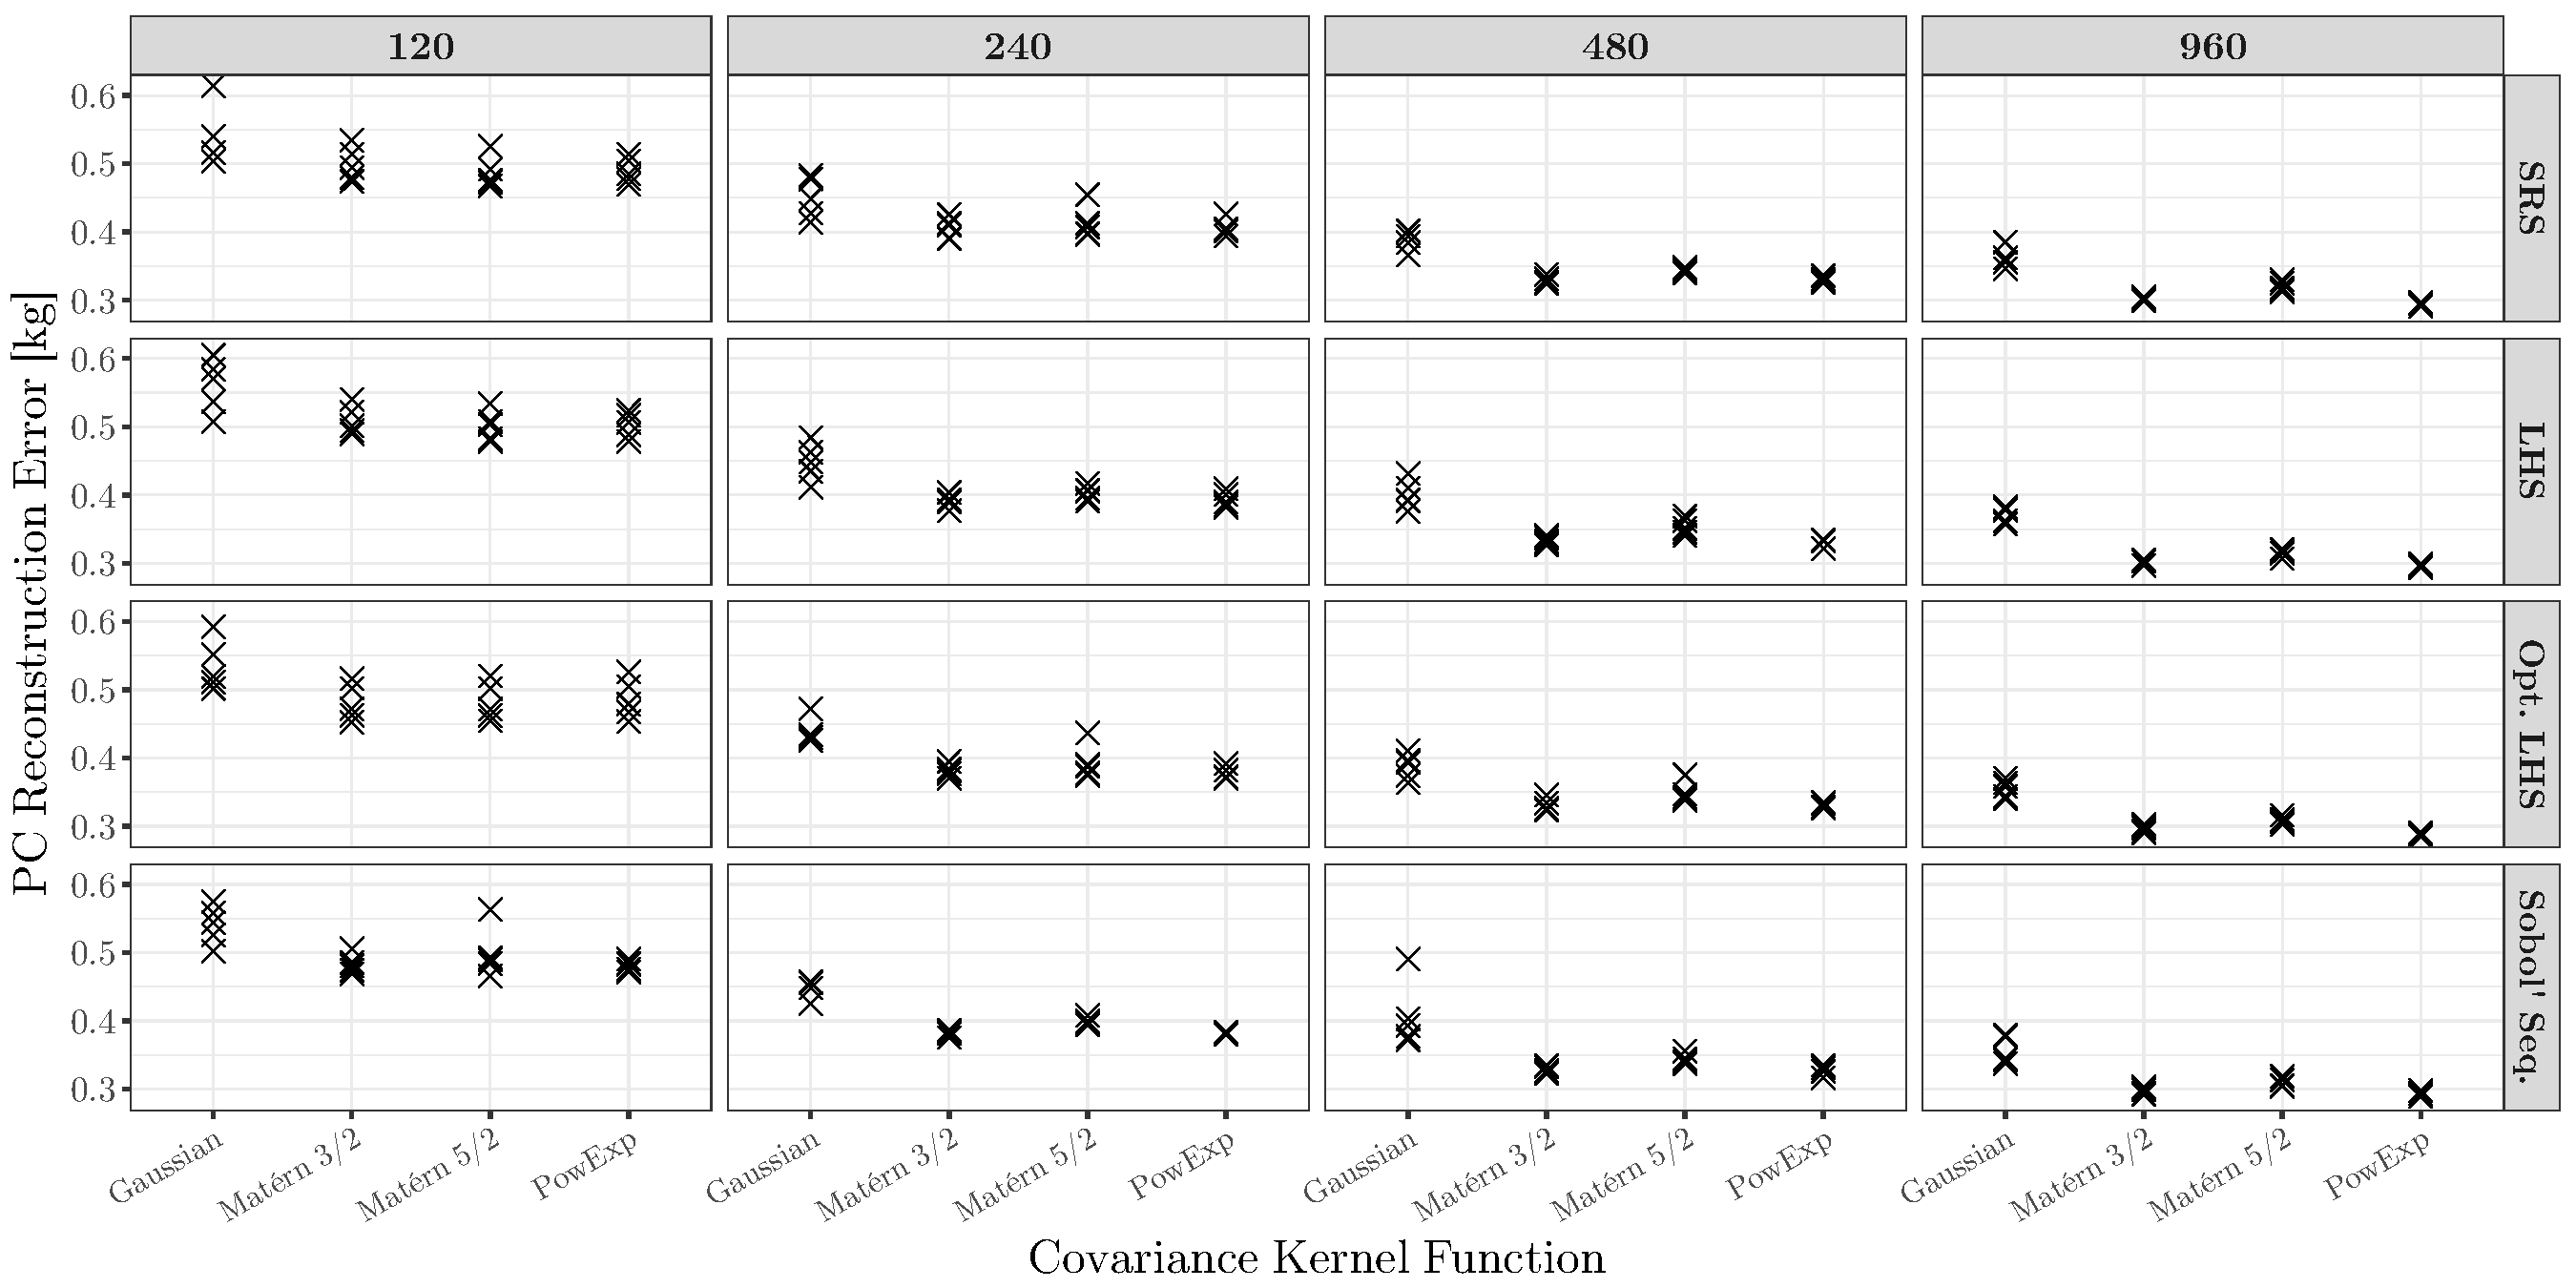
\includegraphics[width=1.0\textwidth]{../figures/chapter4/figures/plotPCGPConstructionCO}
	\caption[The effect of training sample size, experimental design, and covariance function on the predictive performance of GP PC metamodel with respect to the liquid carryover output]{The effect of training sample size, experimental design, and covariance function on the predictive performance (in terms of \gls[hyper=false]{rmse}, of \gls[hyper=false]{gp} \gls[hyper=false]{pc} metamodel with respect to the liquid carryover output.}
	\label{fig:ch4_plot_pc_gp_construction_co}
\end{sidewaysfigure}
\clearpage

%*******************************************************************************************************************************************
\subsection[GP PC Metamodel Testing]{\gls[hyper=false]{gp} \gls[hyper=false]{pc} Metamodel Testing}\label{sub:gp_feba_pca_metamodel_testing}
%*******************************************************************************************************************************************

% Introductory paragraph
Based on the results presented above, a final set of \gls[hyper=false]{gp} metamodels was constructed with a larger training set of $1'920$ samples using a power-exponential covariance kernel function based on a Sobol' sequence (the best options found).
Furthermore, $7$, $10$, and $5$ \glspl[hyper=false]{pc} were used in the reconstruction of the clad temperature, pressure drop, and liquid carryover outputs, respectively.
As such there were $22$ separate \gls[hyper=false]{gp} \gls[hyper=false]{pc} metamodels. 
An additional (i.e., \emph{testing}) dataset of size $5'000$ was then independently generated (with actual \gls[hyper=false]{trace} code runs) 
and used as the basis for testing the predictive performance of the final model.
This additional step was done to avoid any possible bias due to the fact that the validation data set was already used to select the final model.

% Convergence of error measure, test dataset
The validation metric $Q_2$ of the metamodels with respect to the standardized \glspl[hyper=false]{pc} scores computed on the testing dataset converged for all types of output (Fig.~\ref{fig:ch4_plot_q2_pcs}).
In other words, the size of the testing dataset was found to be (or more than) sufficient to assess the predictive performance of the selected metamodel.
\bigfigure[pos=!tbhp,
					 opt={width=1.0\textwidth},
           label={fig:ch4_plot_q2_pcs},
           shortcaption={Convergence of the predictive performance of the metamodel with respect to the standardized \glspl[hyper=false]{pc} scores for each output type}]
{../figures/chapter4/figures/plotQ2PCs}
{Convergence of the predictive performance of the metamodel with respect to the standardized \glspl[hyper=false]{pc} scores for each output type. Shown above are the first $10$ \glspl[hyper=false]{pc} for the clad temperature and pressure drop outputs and the first $5$ \glspl[hyper=false]{pc} for the liquid carryover output. For the clad temperature output, the predictivity coefficient falls below $0.75$ after the first $7$ \glspl[hyper=false]{pc}.}

% The final reconstruction error
There were two main sources of error that dictated the predictive performance of a \gls[hyper=false]{gp} \gls[hyper=false]{pc} metamodel.
The first was due to the representation of the full output dimension only with a few selected \glspl[hyper=false]{pc} (i.e., the dimension reduction) 
and the second was due to the misprediction of the standardized \gls[hyper=false]{pc} scores by the \gls[hyper=false]{gp} metamodel (i.e., the functional approximation).
Fig.~\ref{fig:ch4_plot_rec_error_pred_obs} illustrates these errors by presenting the predicted and observed reconstruction error (in terms of \gls[hyper=false]{rmse}) for each realization in the testing data set.
Note that the \emph{observed} reconstruction error was obtained using the reference standardized \gls[hyper=false]{pc} scores of the testing data set,
while the \emph{predicted} reconstruction error was obtained using the standardized \gls[hyper=false]{pc} scores as predicted by the \gls[hyper=false]{gp} metamodels.
\bigtriplefigure[pos=tbhp,
                 mainlabel={fig:ch4_plot_rec_error_pred_obs},
			           maincaption={Errors, predicted and observed, due to the dimension reduction procedure (\gls[hyper=false]{pca}) and the functional approximation (\gls[hyper=false]{gp}) for the three types of output.},
			           mainshortcaption={Errors, predicted and observed, due to the dimension reduction procedure and the functional approximation for the three types of output.},%
			           leftopt={width=0.31\textwidth},
			           leftlabel={fig:ch4_plot_rec_error_pred_obs_tc},
			           leftcaption={Clad temperature ($TC$) output},
			           midopt={width=0.31\textwidth},
			           midlabel={fig:ch4_plot_rec_error_pred_obs_dp},
			           midcaption={Pressure drop ($DP$) output},
			           rightopt={width=0.31\textwidth},
			           rightlabel={fig:ch4_plot_rec_error_pred_obs_cp},
			           rightcaption={Liquid carryover ($CO$) output},
			           spacing={},
			           spacingtwo={}]
{../figures/chapter4/figures/plotRecErrorPredObsTC}
{../figures/chapter4/figures/plotRecErrorPredObsDP}
{../figures/chapter4/figures/plotRecErrorPredObsCO}

The extend of the $x$-axis signifies the range of error due to the \gls[hyper=false]{pc} truncation.
The farther a data point is from the left, the larger the error is due to the dimension reduction.
On the other hand, the extend of the $y$-axis, specifically the vertical distance between the data points and the line,
signifies the error due to the misprediction of the standardized \glspl[hyper=false]{pc} scores by the \gls[hyper=false]{gp} metamodel.
Data points which are located along the line implied a perfect prediction by the \gls[hyper=false]{gp} metamodel.
The farther a data point is from the line, the larger the error is due to the metamodel approximation.
As can be seen, no data point is located below the line as the truncation error sets the limit of the metamodel predictive performance.
Furthermore, though some data points (i.e., realizations) might be mispredicted and lie over a wide range of value,
the cloud of the data points is only concentrated around a particular range of value.
Table~\ref{tab:ch4_gp_testing} numerically summarizes the results of the testing step.
For comparison the standard deviation of the testing data set for each output is also given.  


\begin{table*}[!bhtp]\centering
\ra{0.9}
\caption{Predictive performance of the selected \gls[hyper=false]{gp} \gls[hyper=false]{pc} metamodel on the testing dataset of size $5'000$}
\label{tab:ch4_gp_testing}
\begin{tabular*}{\textwidth}{@{}rrrrrrrr@{}}\toprule
\multirow{2}{*}{\scriptsize{Output}}&\multirow{2}{*}{\scriptsize{\gls[hyper=false]{pc}\textsubscript{max}}}&\multicolumn{2}{c}{\scriptsize{Predictivity Coefficient}}&\phantom{a}&\multicolumn{2}{c}{\scriptsize{Reconstruction Error}}&\scriptsize{Test Data}\\             
                                                                              \cmidrule{3-4}                                       \cmidrule{6-7}
																			&                                 & \scriptsize{$Q_2$ \gls[hyper=false]{pc}$_1$}&\scriptsize{$Q_2$ \gls[hyper=false]{pc}\textsubscript{max}}&&\scriptsize{\gls[hyper=false]{rmse}\textsubscript{obs}}&\scriptsize{\gls[hyper=false]{rmse}\textsubscript{pred}}&\scriptsize{Std. Dev.}\\ \midrule
\footnotesize{$TC$} & \footnotesize{$7$}  & \footnotesize{$\approx 1.0$}  & \footnotesize{$0.77$} && \footnotesize{$20.17 \, [K] $} & \footnotesize{$22.43 \, [K] $} & \footnotesize{$ 254.0 \, [K] $} \\
\footnotesize{$DP$} & \footnotesize{$10$} & \footnotesize{$\approx 1.0$}  & \footnotesize{$0.74$} && \footnotesize{$55.57 \, [Pa]$} & \footnotesize{$77.95 \, [Pa]$} & \footnotesize{$9200.0 \, [Pa]$} \\
\footnotesize{$CO$} & \footnotesize{$5$}  & \footnotesize{$\approx 1.0$}  & \footnotesize{$0.77$} && \footnotesize{$ 0.16 \, [kg]$} & \footnotesize{$ 0.27 \, [kg]$} & \footnotesize{$  30.4 \, [kg]$} \\
\bottomrule
\end{tabular*}
\end{table*}

%****************************************************
\subsection{Discussion}\label{sub:gp_feba_discussion}
%****************************************************

%Though in principle it was possible to combine all different outputs into a single metamodel through the correlation formulation of the \gls[hyper=false]{pca},
%the approach adopted in this thesis was to construct a separate metamodel for each output.
%\marginpar{pc metamodel}
%It was done to allow for important parameters with respect to each output to retain its prominence.
%Because some parameters were found to be important only with respect to a particular output,
%combining outputs together would have changed the parameter's importance.

% PCA as a dimension reduction tool
The selection of number of \glspl[hyper=false]{pc} to retain is usually done by justifying the amount of total variance explained by the selected \glspl[hyper=false]{pc}.
\marginpar{\gls[hyper=false]{pca} as a dimension reduction tool}
The notion of reconstruction error more intuitively explains the notion of explained variance.
The error represents the difference between the original data and reconstructed data using only a small number of \gls[hyper=false]{pc}.
The series of plots shown in Fig.~\ref{fig:ch4_plot_reconstruction_error} also illustrates the limit of \gls[hyper=false]{pca} as a dimension reduction tool.
The method performs best for the liquid carryover output and worst for the clad temperature output.
The latter is mostly due to the fact that the clad temperature output includes a sharp discontinuity (i.e., quenching).
\gls[hyper=false]{pca}, being a linear transformation, can deal with this strong non-linearities sub-optimally.
That is, significantly large number of \glspl[hyper=false]{pc} are required to bring the reconstruction error to $0$.

% GP PC Metamodel, its limitation
However as indicated in Figs.~\ref{fig:ch4_plot_pc_q2_tc}, \ref{fig:ch4_plot_pc_q2_dp}, and \ref{fig:ch4_plot_pc_q2_co},
constructing a \gls[hyper=false]{pc} metamodel is increasingly difficult for higher \gls[hyper=false]{pc} for all output types.
\marginpar{\gls[hyper=false]{gp} \gls[hyper=false]{pc} metamodel, limitation}
In other words, as the relationship between model parameters and the standardized \gls[hyper=false]{pc} scores becomes increasingly non-linear, 
large number of training samples are required to train the \gls[hyper=false]{gp} metamodel to attain a decent predictive performance.
At the same time, the benefit of adding additional \gls[hyper=false]{pc} becomes increasingly marginal (Fig.~\ref{fig:ch4_plot_reconstruction_error}).
In addition to that, some degree of error should be expected in the prediction of the \gls[hyper=false]{pc} scores by the metamodel, especially the higher ones.
As such, unless the score is perfectly predicted, this error might offset the potential benefit of adding additional \gls[hyper=false]{pc} for the reconstruction.

% GP PC Metamodel, errors in context
A pragmatic approach is thus to choose the number of retained \glspl[hyper=false]{pc} based on some target error put in context and/or number of \gls[hyper=false]{trace} runs that can be afforded.
\marginpar{\gls[hyper=false]{gp} \gls[hyper=false]{pc} metamodel, errors in context}
For the clad temperature output,
retaining $7$ \glspl[hyper=false]{pc} for the \gls[hyper=false]{gp} \gls[hyper=false]{pc} metamodel gives reconstruction error of $\approx 22 \, [K]$ (\gls[hyper=false]{rmse}).
This value is small in comparison with the output standard deviation of the test data itself, $254 \, [K]$.
The same approach applies to the pressure drop output ($10$ \glspl[hyper=false]{pc} gives reconstruction error of $\approx 78 \, [Pa]$, compared with test data standard deviation of $9200 \, [Pa]$);
and the liquid carryover output ($10$ \glspl[hyper=false]{pc} gives reconstruction error of $0.27 \, [kg]$, compared with the test data standard deviation of $30.4 \, [kg]$).
Note that those numbers are based on training samples of size $1'920$ and testing samples of size $5'000$.

% The effects of training sample size, experimental design, and covariance function
Another important finding in this study is the major importance of the training sample size on the predictive performance of the \gls[hyper=false]{gp} \gls[hyper=false]{pc} metamodel.
\marginpar{the effects of training sample size, experimental design, and covariance function}
The choice of covariance function has some effect in the predictive performance and its variation across replication insofar the choice is between the smoother ones (e.g., the Gaussian, the Mate\'rn $5/2$) and the less smooth ones (e.g., the power-exponential, the Mate\'rn $3/2$), 
with the performance of the smoother kernels tend to be more variable.
The choice of experimental design, on the other hand, has a small to negligible effect on the predictive performance across different sample sizes, covariance functions, and replications.

% GP PC Metamodel, a statistical metamodel
It is also worth noting that that a \gls[hyper=false]{gp} \gls[hyper=false]{pc} metamodel is a global statistical metamodel.
\marginpar{\gls[hyper=false]{gp} \gls[hyper=false]{pc} metamodel, a statistical metamodel}
This implies that its predictive performance is defined over all output space (such as through the use of $Q_2$ and \gls[hyper=false]{rmse} as the validation metrics.) and over many realizations.
That is, a good metamodel accurately predicts the output at arbitrary input, \emph{on average}.
This also means that the metamodel has to some extent a ``hit-and-miss'' property: 
most realizations are accurately predicted, some realizations can be mispredicted, and some small proportion of that can be grossly mispredicted as was illustrated in Fig.~\ref{fig:ch4_plot_rec_error_pred_obs}.
Fig.~\ref{fig:ch4_plot_hit_and_miss} illustrates this idea further for the clad temperature output.
\normdoublefigure[pos=!tbhp,
                 mainlabel={fig:ch4_plot_hit_and_miss},
								 mainshortcaption={\gls[hyper=false]{gp} \gls[hyper=false]{pc} metamodel is a global statistical metamodel which gives global accurate prediction \emph{on average}.},
                 maincaption={\gls[hyper=false]{gp} \gls[hyper=false]{pc} metamodel is a global statistical metamodel which gives global accurate prediction \emph{on average}. Some realizations are better than the others, due to both the limitation in the approximations incurred by using \gls[hyper=false]{pc} and \gls[hyper=false]{gp} (e.g., around quenching). Solid and dashed lines are \gls[hyper=false]{trace} runs and \gls[hyper=false]{gp} \gls[hyper=false]{pc} prediction.},
                 leftopt={width=0.475\textwidth},
                 leftlabel={fig:ch4_plot_hit_and_miss_2},
                 leftcaption={example of better prediction},
                 rightopt={width=0.475\textwidth},
                 rightlabel={fig:ch4_plot_hit_and_miss_1},
                 rightcaption={example of worse prediction}]
{../figures/chapter4/figures/plotHitAndMiss_1}
{../figures/chapter4/figures/plotHitAndMiss_2}

% Computational cost
A prediction made by a fully specified (or trained) \gls[hyper=false]{gp} metamodel is, according to Eq.~(\ref{eq:mean_sk}), a straightforward matrix operation.
\marginpar{Computational cost}
In \texttt{R} through the package \texttt{DiceKriging}, the operation to predict a standardized \gls[hyper=false]{pc} score for an arbitrary input takes about $0.05 \, [s]$.
For a full output reconstruction, this operation has to be repeated for multiple \glspl[hyper=false]{pc} scores before multiplied with the \gls[hyper=false]{pc} loadings.
The actual time required for this full reconstruction is specific to a particular implementation and to particular programming language.
Though no thorough investigation was carried out, 
the cost of evaluating the metamodel for an arbitrary input is still expected to be much less than running an actual \gls[hyper=false]{trace} simulation ($6 - 14 \, [min]$).
For instance, the most naive implementation in \texttt{R} involving loops takes, on average, about $< 5 \, [s]$ to predict and reconstruct all outputs (clad temperature, pressure drop, and liquid carryover) for a given input.
However, it is also important to take into account the computational cost required to train, validate, and test the metamodel.
The training, validation, and testing data have to be generated from actual \gls[hyper=false]{trace} runs.
Additionally, the model fitting step during training is an optimization problem that becomes computationally expensive for large training samples of large dimension (large number of input parameters).
Again, further study is required to have a more quantitative cost measure.
